\chapter{Portierung von NUMA-Locks auf verteilten Speicher}
\label{ch:portierung}

Es gibt einige Locks für Systeme mit gemeinsamem Speicher,
die die Unterschiede zwischen Zugriffen auf lokalen und entfernten Speicher bei \gls{numa} berücksichtigen
und Fairness opfern,
um höhere Geschwindigkeiten zu erreichen.
Obwohl die Geschwindigkeitsunterschiede von Speicherzugriffen in verteilten Systemen noch deutlich ausgeprägter sind,
wird diese Technik dort kaum genutzt.
Dabei ähneln sich Speicherzugriffe auf gemeinsamem Speicher und \gls{rma} auf verteilten Systemen stark.
In diesem Kapitel werden daher einige \gls{numa}-Locks untersucht
und wenn möglich auf verteilten Speicher portiert.

\section{Delegierende Locks}
\label{sec:delegation_locks}

Neben klassischen Locks,
die in \autoref{sec:synchronisierung_in_parallelen_programmen} beschrieben wurden,
gibt es bei Systemen mit gemeinsamem Speicher das Konzept von delegierenden Locks,
welche zum Teil auch \gls{numa} berücksichtigen \cite{OyamaAlg} \cite{FlatCombining} \cite{P-Sim} \cite{H-Sync} \cite{RCL} \cite{shared-mem-delegation} \cite{SANL} \cite{DYLOCK}.
Die Idee dabei ist,
dass ein oder mehrere Prozesse als Server agieren
und kritische Abschnitte für alle anderen Client-Prozesse ausführen.
Client-Prozesse schicken dafür Anfragen an den Server,
in denen der auszuführende kritische Abschnitt,
sowie die notwendigen Parameter enthalten sind
und warten auf eine Antwort des Servers,
die zeigt,
dass der kritische Abschnitt ausgeführt wurde.

Unterschieden wird dabei zwischen statischen und dynamischen Locks,
je nachdem,
ob ein oder mehrere fest bestimmte Prozesse als Server dienen,
oder jeder Prozess dynamisch für eine gewisse Zeit zu einem Server werden kann.

Delegierende Locks haben in Systemen mit gemeinsamem Speicher den großen Vorteil,
dass die Daten,
die durch den Lock geschützt werden
und auf die im kritischen Abschnitt zugegriffen wird,
immer von demselben Prozess (dem Server-Prozess) verwendet werden.
Damit liegen sie dort typischerweise in lokalen \gls{Zwischenspeicher}n vor,
wodurch besonders schnell auf sie zugegriffen werden kann.

Ein Nachteil von delegierenden Locks ist allerdings,
dass sie nicht dieselbe Programmierschnittstelle nutzen können
wie klassische Locks,
weil sie Zugriff auf alle Parameter des kritischen Abschnitts benötigen
und der kritische Abschnitt selbst eine eigene Funktion sein muss,
damit der Server-Prozess diese direkt aufrufen kann.
Ein Programm von klassischen Locks auf delegierende Locks umzustellen,
kann daher sehr aufwendig sein.

Bei verteiltem Speicher besteht darüber hinaus das Problem,
dass Prozesse im kritischen Abschnitt auch auf private Daten zugreifen können,
die nicht über ein \gls{Fenster} veröffentlicht wurden.
In so einem Fall ist es für einen anderen Prozess gar nicht möglich,
den kritischen Abschnitt auszuführen.
Delegierende Locks eignen sich daher nicht für eine Portierung auf verteilten Speicher.
Außerdem kommt der Hauptvorteil von delegierenden Locks,
dass die Daten des kritischen Abschnitts meist schon im \gls{Zwischenspeicher} des Server-Prozesses liegen,
bei verteiltem Speicher nicht zum Tragen,
da in \gls{mpi} die Daten von entfernen Prozessen nicht automatisch zwischengespeichert werden.

Das Konzept der Delegierung an einen Server-Prozess passt allerdings sehr gut zu \gls{message passing}
und die hier beschriebenen Probleme lassen sich leicht vermeiden,
wenn ein Programm speziell dafür entwickelt wird.
Daher eignet sich dieses Konzept möglicherweise,
um parallele Datenstrukturen,
z.~B. Warteschlangen (engl. \textit{Queues}),
für verteilte Systeme zu entwickeln.

\section{RH-Lock}
\label{sec:rh-lock}

Der RH-Lock \cite{RH-Lock} ist der erste bekannte Lock
der \gls{numa} berücksichtigt,
um eine bessere Performance zu erzielen.
Er besteht aus einem \gls{tts}-Lock \cite{TTS-Lock} mit exponentiellem Backoff \cite{backoff} (siehe \autoref{sec:spin_locks}) pro \gls{numa}-Knoten.
Da der RH-Lock nur zwei \gls{numa}-Knoten unterstützt,
sind es also immer zwei \gls{tts}-Locks.

Statt einer \textit{Test-and-Set}-Operation,
nutzen die \gls{tts}-Locks für lokale Akquisitionen keine \gls{tas}-,
sondern eine \textit{swap}-Operation,
da der Lock-Status nicht nur die Werte \enquote{FREE} und \enquote{ACQUIRED} annehmen kann.
Wenn der Lock nicht verfügbar ist,
enthält der Lock-Status stattdessen die eindeutige ID des Prozesses,
der zuletzt mit einer \textit{swap}-Operation versucht hat,
den Lock zu akquirieren,
oder den Status \enquote{REMOTE},
wenn zuletzt ein Prozess des anderen \gls{numa}-Knotens den Lock erfolgreich akquiriert hat.

Durch die IDs hat ein Prozess die Möglichkeit,
den Lock mit einer \gls{cas}-Operation nur dann global freizugeben,
wenn der Status immer noch seine ID enthält.
Wenn diese \gls{cas}-Operation fehlschlägt,
muss es innerhalb seines \gls{numa}-Knotens einen anderen Prozess geben,
der auf den Lock wartet.
In diesem Fall wird der Lock mit dem Status \enquote{L\_FREE} nur lokal,
also für Prozesse im selben \gls{numa}-Knoten freigeben.

Liest ein Prozess den Status \enquote{REMOTE},
weiß er,
dass er die Speicheradresse des \gls{tts}-Locks
des jeweils anderen \gls{numa}-Knotens
für die Akquisition
nutzen muss.
Durch die \textit{swap}-Operation
sieht nur der erste Prozess eines \gls{numa}-Knotens den \enquote{REMOTE} Status.
Alle weiteren Prozesse sehen die ID ihres Vorgängers
und warten auf den lokalen \gls{tts}-Lock.

Um einen entfernten \gls{tts}-Lock zu akquirieren,
prüft ein Prozess,
anders als bei seinem lokalen \gls{tts}-Lock,
nicht zuerst mit einer Lese-Operation,
ob der Lock frei ist.
Der Lock funktioniert in diesem Fall also eher wie ein \gls{tas}-Lock (vgl. \autoref{fig:tas_code}) mit Backoff.
Dadurch,
dass entfernte Zugriffe langsamer sind,
hätte ein entfernter Prozess sonst kaum eine Chance,
den Lock zu akquirieren,
da er deutlich länger braucht,
um darauf zu reagieren,
dass der Lock frei ist.
Stattdessen versucht ein Prozess immer direkt mit einer \gls{cas}-Operation,
den entfernten Lock zu akquirieren.
Hierbei wird \gls{cas},
statt \textit{swap} genutzt,
da der entfernte Lock nur akquiriert werden soll,
wenn er den Status \enquote{FREE},
nicht aber z.~B. den Status \enquote{L\_FREE} hat.

Um \gls{Verhungern} zu vermeiden,
% also dass immer wieder Prozesse desselben \gls{numa}-Knotens den Lock akquirieren
% und die anderen Prozesse für immer warten,
setzt der RH-Lock einen Zufallszahlengenerator ein
und gibt mit konfigurierbarer Wahrscheinlichkeit den Lock global frei,
selbst wenn es einen lokalen wartenden Prozess gibt,
sodass alle Prozesse die Möglichkeit haben,
den Lock zu akquirieren.

\clearpage

\subsection{Portierung und Optimierung des RH-Locks}

Das größte Problem des RH-Locks für eine Portierung auf verteilten Speicher ist,
dass der Lock nur zwei \gls{numa}-Knoten unterstützt.
Es ist aber eher selten,
dass ein verteiltes System aus nur zwei Knoten besteht.
Dieses Problem lässt sich z.~B. beheben,
indem man den \enquote{REMOTE} Status erweitert
und dort zusätzlich die ID des entfernten Prozesses codiert,
in dessen Speicher der \gls{tts}-Lock ist.
Für die Portierung werden hierfür negative Zahlen verwendet ($-id - 1$ um die ID 0 zu unterstützen),
da Prozess IDs typischerweise positiv sind.
Somit signalisiert eine positive Zahl,
dass der Prozess lokal warten muss
und eine negative Zahl,
dass der Prozess auf den \gls{tts}-Lock
im Speicher des entfernten Prozesses mit der zugehörigen positiven ID warten muss.

Bei mehr als zwei Knoten kann es nun allerdings passieren,
dass ein Prozess auf Knoten $a$ einen \enquote{REMOTE} Wert liest,
der ihn auf Knoten $b$ verweist,
obwohl Knoten $b$ den Lock gar nicht mehr hat,
da inzwischen ein Prozess von Knoten $c$ den Lock akquiriert hat.
Daher kann ein Prozess nicht mehr einfach darauf warten,
dass der \gls{tts}-Lock des anderen Knotens frei wird,
sondern muss auch dort prüfen,
ob es sich um einen \enquote{REMOTE} Wert handelt,
der ihn weiter verweist.
Bei einem freien RH-Lock muss ein Prozess so im schlimmsten Fall jeden anderen \gls{tts}-Lock fragen,
bis er den richtigen findet.
Dieser Overhead steigt demnach linear mit der Anzahl der beteiligten Knoten.

Beim RH-Lock gehen die meisten Speicherzugriffe auf den lokalen \gls{tts}-Lock des \gls{numa}-Knotens,
was gut ist,
da lokale Zugriffe schneller als entfernte sind.
Dabei handelt es sich vor allem um die Lese-Operation,
mit der ermittelt wird,
ob der Lock frei ist.
Da es sich um einen lokalen Zugriff handelt,
kann genau diese Operation ohne \gls{rma} mit einem schnelleren direkten Speicherzugriff implementiert werden,
wenn für die lokale Kommunikation ein \gls{Fenster} auf den gemeinsamen Speicher erstellt wurde
(vgl. \autoref{sec:mpi_shared_mem}).
Dabei ist zu beachten,
dass in der Warteschleife \texttt{MPI\_Iprobe} aufgerufen wird,
um Programmfortschritt zu garantieren (vgl. \autoref{sec:mpi_fortschritt}).

\subsection{Evaluation des RH-Locks}

Da die Warteschleife einen Aufruf von \texttt{MPI\_Iprobe} enthalten muss,
um Programmfortschritt zu garantieren,
ist sie deutlich langsamer
als eine leere Warteschleife,
wie sie in \cite{RH-Lock} genutzt wird.
Außerdem ist die Latenz von Zugriffen auf entfernten Speicher
in einem verteilten System deutlich höher
als in einem System mit gemeinsamem \gls{numa}-Speicher,
da der Zugriff über das Netzwerk gehen muss.
Allein aus diesem Grund ist die Frequenz,
mit der versucht wird,
einen entfernten \gls{tts}-Lock zu akquirieren,
deutlich geringer.
Aus diesen beiden Gründen können nicht einfach dieselben Werte für Backoff (vgl. \autoref{sec:spin_locks}) verwendet werden
wie in \cite{RH-Lock}.

Durch die hohe Latenz von entfernten Speicherzugriffen,
ist die Frequenz dieser Zugriffe während des Wartens auf einen entfernten \gls{tts}-Lock bereits so niedrig,
dass zusätzlicher Backoff keine Verbesserung bringt,
sondern entfernte Prozesse nur unfair benachteiligt.
Der initiale und maximale Backoff für das entfernte Akquirieren werden daher in der Evaluation auf 0 gesetzt,
wodurch der Backoff deaktiviert wird.

Für Zugriffe auf den lokalen \gls{tts}-Lock hingegen ist Backoff weiterhin sinnvoll.
Durch die Verwendung von \texttt{MPI\_Iprobe}
sind die optimalen Werte aber deutlich geringer
als in \cite{RH-Lock}.
Als maximaler Backoff werden lokal 16, 32 und 64 Iterationen evaluiert,
da ungefähr bei 32 Backoff-Iterationen ein lokales Optimum
bei einer durchschnittlichen Wartezeit von 1~\textmu{s} im \gls{wbab} liegt.
Da diese Maximalwerte so klein sind,
wird als Minimalwert immer 1 verwendet.
So erreicht ein Prozess spätestens nach dem 7. Zugriff auf den \gls{tts}-Lock die maximale Wartezeit von $2^6 = 64$ Iterationen.

Wie bereits in \autoref{sec:spin_locks} erläutert,
hängt die optimale Backoff-Konfiguration von der Geschwindigkeit des verwendeten Systems,
aber auch von dem konkreten Szenario (Länge des kritischen Abschnitts, Anzahl der Prozesse) ab.
Es ist also möglich,
dass in manchen Szenarien eine andere Konfiguration besser wäre.
Die Optimierung auf eine durchschnittliche Wartezeit von 1~\textmu{s} im \gls{wbab} ist zwar willkürlich,
liefert aber zumindest deutlich bessere Ergebnisse
als eine einfache Wiederverwendung der Konfiguration aus \cite{RH-Lock}.

Neben dem Backoff ist beim RH-Lock auch die Fairness konfigurierbar.
Hier muss eingestellt werden,
mit welcher Wahrscheinlichkeit trotz lokalen Nachfolgers der Lock global freigegeben wird.
In dieser Arbeit werden für einen maximalen lokalen Backoff von 32,
wie in \cite{RH-Lock} die Fairnessfaktoren 1, 2 \& 100 evaluiert.
D.~h. der Lock wird bei einem lokalen Nachfolger trotzdem mit einer Wahrscheinlichkeit von $1$, $\frac{1}{2}$ oder $\frac{1}{100}$ global freigegeben.
Bei einem maximalem lokalen Backoff von 16 und 64 ist der RH-Lock in dieser Arbeit immer maximal fair (also mit einem Fairnessfaktor von 1) eingestellt.

\begin{benchmark}[h]
    \begin{subfigure}{.5\textwidth}
        \includegraphics[width=\textwidth]{benchmarks/intelmpi/rh/UPB-lock_count=1000-latency}
        \caption{Iterationsdauer in \textmu{s}}
        \label{ben:rh_upb_latency}
    \end{subfigure}
    \begin{subfigure}{.5\textwidth}
        \includegraphics[width=\textwidth]{benchmarks/intelmpi/rh/UPB-lock_count=1000-throughput}
        \caption{Durchsatz in Mio/s}
        \label{ben:rh_upb_throughput}
    \end{subfigure}
    \caption{UPB des RH-Locks}
    \label{ben:rh_upb}
\end{benchmark}

\autoref{ben:rh_upb_latency} zeigt,
wie lange es dauert,
einen freien RH-Lock zu akquirieren,
im Vergleich zum optimierten D-MCS-Lock aus \autoref{sec:optimierung_dmcs} und RMA-MCS.
Die Backoff- und Fairness-Konfiguration spielt für diesen Benchmark keine Rolle,
da alle Locks frei sind,
somit wird hier nur ein RH-Lock gezeigt.
Anders als bei den anderen \gls{upb}-Evaluationen,
sind hier alle neun Szenarien (vgl. \autoref{tab:upb_szenarien}) separat aufgeführt.
Beim RH-Lock macht es nämlich einen Unterschied,
welcher Prozess den Lock als Letztes besaß.

Während es bei den optimierten D-MCS- und RMA-MCS-Locks vor allem entscheidend ist,
wie weit der akquirierende Prozess vom Hauptprozess entfernt ist,
also ob es ein a-, b- oder c-Szenario ist,
ist es beim RH-Lock vor allem wichtig,
ob der Vorgängerprozess auf demselben Knoten lief,
also ob es ein 1er, 2er oder 3er-Szenario ist.
Das liegt daran,
dass es beim RH-Lock keinen globalen Hauptprozess gibt.
Alle Rechenknoten sind beim RH-Lock äquivalent.
Es gibt allerdings auf jedem Rechenknoten einen lokalen Hauptprozess,
in dessen Speicher sich der \gls{tts}-Lock befindet.

\clearpage

Überraschenderweise lässt sich ein RH-Lock schneller durch einen lokalen Hauptprozess akquirieren.
\autoref{ben:rh_upb} zeigt deutlich,
dass der RH-Lock in den b-Szenarien (Prozess ist kein Hauptprozess) deutlich langsamer ist
als in den a-Szenarien (Prozess ist ein Hauptprozess).
In den c-Szenarien ist das Bild gemischt.
Die c-Szenarien zeigen die Performance,
wenn der akquirierende Prozess nicht auf dem Hauptknoten läuft.
D-MCS und RMA-MCS sind hier deutlich langsamer als in den anderen Szenarien,
da sie entferne Zugriffe auf den Hauptknoten benötigen.
Beim RH-Lock gibt es aber keinen Hauptknoten,
sodass er sich in c-Szenarien genauso verhält
wie in den anderen.
Das gemischte Bild entsteht dadurch,
dass der akquirierende Prozess in Szenario 1c und 3c ein lokaler Hauptprozess ist,
in 2c aber nicht.
Daher ist die Performance des RH-Locks in Szenario 1c identisch zu der in 1a,
in 2c identisch zu der in 2b
und in 3c identisch zu der in 3a.

% Tatsächlich sieht man,
% dass auch D-MCS und RMA-MCS in Szenario 2c etwas langsamer sind
% als in 1c und 3c.
% Bei RMA-MCS könnte das daran liegen,
% dass auch dieser lokale Hauptprozesse nutzt.
% Bei D-MCS ist das aber nicht der Fall.
% Hier greift der akquirierende Prozess in allen drei c-Szenarien nur auf seinen eigenen
% und den entfernten Speicher des globalen Hauptprozesses zu.
% Warum die Performance von D-MCS in Szenario 2c schlechter ist,
% ist also nicht klar.

\begin{benchmark}[h]
    \begin{subfigure}{.5\textwidth}
        \includegraphics[width=\textwidth]{benchmarks/intelmpi/rh/ECSB-latency}
        \caption{Iterationsdauer in \textmu{s}}
        \label{ben:rh_ecsb_latency}
    \end{subfigure}
    \begin{subfigure}{.5\textwidth}
        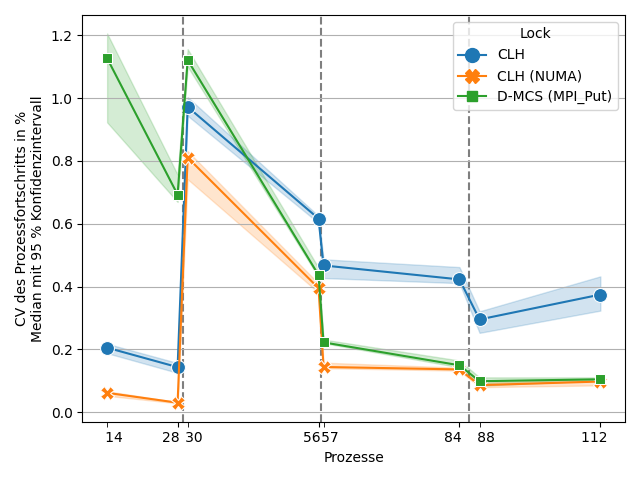
\includegraphics[width=\textwidth]{benchmarks/intelmpi/rh/ECSB-fairness}
        \caption{Fairness: CV des Fortschritts in \%}
        \label{ben:rh_ecsb_fairness}
    \end{subfigure}
    \caption{ECSB des RH-Locks}
    \label{ben:rh_ecsb}
\end{benchmark}

\autoref{ben:rh_ecsb} zeigt den \gls{ecsb} für die verschiedenen Konfigurationen des RH-Locks,
den D-MCS und RMA-MCS.
Dabei steht \enquote{lbx} für \enquote{lokales Backoff-Maximum} und \enquote{f} für \enquote{Fairnessfaktor}.
In \autoref{ben:rh_ecsb_latency} sieht man,
dass bei mehreren Rechenknoten alle RH-Locks (außer mit lbx=16) schneller sind
als der D-MCS-Lock.
Dieser Vorteil wird aber mit erheblichen Fairnessproblemen erkauft,
wie \autoref{ben:rh_ecsb_fairness} zeigt.
Während D-MCS und RMA-MCS sehr fair sind (ohne erkennbare Abweichung von 0~\%),
haben alle RH-Locks extrem schlechte Fairnesswerte,
auf einem Rechenknoten sogar einen Variationskoeffizienten von bis zu 460~\%.
Bei mehr Rechenknoten wird es zwar etwas besser,
der fairste RH-Lock fällt bei 112 Prozessen auf einen Variationskoeffizienten von knapp unter 40~\%,
aber sie bleiben ziemlich unfair.
Da im \gls{ecsb} Prozesse außerhalb des kritischen Abschnitts nichts tun müssen,
kann derselbe Prozess den Lock immer wieder akquirieren
und so anderen Prozessen zuvorkommen.
Daher ist die Fairness in diesem Benchmark besonders schlecht.

\autoref{ben:rh_ecsb_fairness} zeigt auch,
dass die Fairness auf mehreren Rechenknoten noch weiter abnimmt,
wenn andere Werte für den Fairnessfaktor verwendet werden (2 und 100).
Die Geschwindigkeit in \autoref{ben:rh_ecsb_latency} nimmt dafür weiter zu.
Man hat also hier die Möglichkeit,
noch mehr Fairness für Geschwindigkeit zu opfern.
Trotzdem kommt der RH-Lock mit keiner der Konfigurationen an die Geschwindigkeit von RMA-MCS heran,
welcher obendrein auch noch sehr fair ist.
Dieser hat allerdings in diesem Vergleich
die mit Abstand schlechteste Performance
bei nur einem Rechenknoten (auf 14 und 28 Prozessen).

\begin{benchmark}[h]
    \begin{subfigure}{.5\textwidth}
        \includegraphics[width=\textwidth]{benchmarks/intelmpi/rh/CCWB-processes=112-latency}
        \caption{Iterationsdauer in \textmu{s}}
        \label{ben:rh_ccwb_112_latency}
    \end{subfigure}
    \begin{subfigure}{.5\textwidth}
        \includegraphics[width=\textwidth]{benchmarks/intelmpi/rh/CCWB-processes=112-latency-max}
        \caption{Iterationsdauer in \textmu{s}}
        \label{ben:rh_ccwb_112_latency_max}
    \end{subfigure}
    \begin{subfigure}{.5\textwidth}
        \includegraphics[width=\textwidth]{benchmarks/intelmpi/rh/CCWB-processes=112-fairness}
        \caption{Fairness: CV des Fortschritts in \%}
        \label{ben:rh_ccwb_112_fairness}
    \end{subfigure}
    \begin{subfigure}{.5\textwidth}
        \includegraphics[width=\textwidth]{benchmarks/intelmpi/rh/CCWB-processes=112-contention}
        \caption{Konkurrenz in \%}
        \label{ben:rh_ccwb_112_contention}
    \end{subfigure}
    \caption{CCWB des RH-Locks mit 112 Prozessen}
    \label{ben:rh_ccwb_112}
\end{benchmark}

Auch beim \gls{ccwb} sieht man in \autoref{ben:rh_ccwb_112_fairness},
dass der RH-Lock deutlich unfairer ist
als D-MCS und RMA-MCS.
Vor dem Equilibrium sind alle Locks gleich fair.
Während bei D-MCS und RMA-MCS die Fairness ab dem Equilibrium besser wird,
da Prozesse sich bei einer \gls{Konkurrenz} von 100~\% in eine Warteschlange mit beschränkter Fairness einreihen müssen,
wird die Fairness des RH-Locks in allen Konfigurationen immer schlechter.
Die Fairness ist aber um ein Vielfaches besser
als im \gls{ecsb},
da der \gls{ccwb} ein deutlich realistischeres Szenario implementiert,
bei dem Prozesse auch außerhalb des kritischen Abschnitts Arbeit ausführen.

Die bessere Fairness bringt aber leider auch eine schlechtere Geschwindigkeit mit sich.
Im Gegensatz zum \gls{ecsb} ist der RH-Lock hier nur mit einem \enquote{lbx} von 16 schneller
als der D-MCS-Lock.
Und das auch nur bei einer kritischen Arbeit von 4 und 5.
Beim \gls{ecsb} war es genau anders herum:
Dort war der RH-Lock nur mit einem \enquote{lbx} von 16 langsamer als der D-MCS-Lock.
Da die Locks in \autoref{ben:rh_ccwb_112_latency} so dicht beieinanderliegen,
dass sie schwer zu unterscheiden sind,
zeigt \autoref{ben:rh_ccwb_112_latency_max} eine Nahaufnahme der Performance bei einer kritischen Arbeit von 5.
Diese Nahaufnahme zeigt überraschenderweise,
dass ein höherer Fairnessfaktor im \gls{ccwb} zu einem langsameren Lock führt.
Auch das war im \gls{ecsb} genau umgekehrt.
Die Idee des Fairnessfaktors ist es eigentlich,
Fairness zu opfern,
um die Geschwindigkeit zu verbessern.
Der \gls{ccwb} zeigt aber,
dass in einem realistischen Szenario durch einen höheren Fairnessfaktor sowohl Fairness
als auch Geschwindigkeit geopfert werden.

Der Grund hierfür ist wahrscheinlich,
dass die Lock-Freigabe aus einer zusätzlichen \gls{cas}-Operation besteht,
wenn sich der Prozess unfair verhält,
also den Lock nur lokal freigibt.
Der Status darf nur auf \enquote{L\_FREE} gesetzt werden,
wenn es einen lokalen Nachfolger gibt.
Sonst könnte es zu einem Deadlock kommen.
Daher wird bei der unfairen Freigabe der Status erst gesetzt,
wenn die \gls{cas}-Operation fehlschlägt,
die den Lock global freigeben würde.
Die zusätzliche \gls{cas}-Operation liegt auf dem kritischen Pfad
und schlägt bei einer kritischen Arbeit von 5 immer fehl,
da die \gls{Konkurrenz} bei 100~\% liegt (vgl. \autoref{ben:rh_ccwb_112_contention}).
Die faire Freigabe hingegen besteht nur aus einer Operation,
die den Status immer auf \enquote{FREE} setzt.

Obwohl die zusätzliche \gls{cas}-Operation auf lokalen Speicher zugreift,
kann sie nicht mit C++ \texttt{std::atomic} implementiert werden,
da auf dieselbe Speicheradresse auch entfernt zugegriffen wird.
Es muss also ein langsamer \gls{rma}-Zugriff verwendet werden.
Auf gemeinsamem Speicher wird die zusätzliche \gls{cas}-Operation dadurch ausgeglichen,
dass durch eine lokale Lockübergabe die Daten,
auf die der Nachfolgerprozess im kritischen Abschnitt zugreift,
bereits im \gls{Zwischenspeicher} vorliegen.
Bei verteiltem Speicher gibt es allerdings keine \gls{Zwischenspeicher} für entfernten Speicher,
sodass dieser Vorteil hier nicht zum tragen kommt.

\begin{benchmark}[h]
    \begin{subfigure}{.5\textwidth}
        \includegraphics[width=\textwidth]{benchmarks/intelmpi/rh/WBAB-processes=112,mpi_progress=1-latency}
        \caption{Iterationsdauer in \textmu{s}}
        \label{ben:rh_wbab_112_latency}
    \end{subfigure}
    \begin{subfigure}{.5\textwidth}
        \includegraphics[width=\textwidth]{benchmarks/intelmpi/rh/WBAB-processes=112,mpi_progress=1-fairness}
        \caption{Fairness: CV des Fortschritts in \%}
        \label{ben:rh_wbab_112_fairness}
    \end{subfigure}
    \begin{subfigure}{.5\textwidth}
        \includegraphics[width=\textwidth]{benchmarks/intelmpi/rh/WBAB-processes=112,mpi_progress=1-overhead}
        \caption{Overhead in \textmu{s}}
        \label{ben:rh_wbab_112_overhead}
    \end{subfigure}
    \begin{subfigure}{.5\textwidth}
        \includegraphics[width=\textwidth]{benchmarks/intelmpi/rh/WBAB-processes=112,mpi_progress=1-contention}
        \caption{Konkurrenz in \%}
        \label{ben:rh_wbab_112_contention}
    \end{subfigure}
    \caption{WBAB des RH-Locks mit 112 Prozessen}
    \label{ben:rh_wbab_112}
\end{benchmark}

\autoref{ben:rh_wbab_112} zeigt die Ergebnisse des RH-Locks im \gls{wbab}.
Genau wie im \gls{ccwb} führt auch beim \gls{wbab} ein höherer Fairnessfaktor
zu einem langsameren Lock.
Bei der Geschwindigkeit in \autoref{ben:rh_wbab_112_latency} erreicht keiner der RH-Locks mehr die Performance von D-MCS,
sobald Prozesse außerhalb des kritischen Abschnitts warten.
Dafür zeigt \autoref{ben:rh_wbab_112_overhead} aber,
dass bei geringer \gls{Konkurrenz}
(Wartezeit von 8~\textmu{s} bis 32~\textmu{s})
der RH-Lock in allen Konfigurationen schneller ist
als D-MCS und sogar RMA-MCS.
Das passt auch zu den Ergebnissen aus \autoref{ben:rh_upb},
nach denen ein freier RH-Lock schneller als D-MCS und RMA-MCS akquiriert werden kann,
wenn der Prozess nicht auf dem Hauptknoten läuft.
Der RH-Lock hat hier den Vorteil,
dass keine MCS-Warteschlangen initialisiert werden müssen.

In \autoref{ben:rh_wbab_112_fairness} sieht man noch einmal die extreme Unfairness des RH-Locks,
wenn Prozesse keine Wartezeit außerhalb des kritischen Abschnitts haben,
die auch der \gls{ecsb} gezeigt hat.
Diese wird bereits bei geringer Wartezeit deutlich besser,
bleibt aber suboptimal,
bis die \gls{Konkurrenz} bei einer Wartezeit von 8~\textmu{s} stark abfällt
(vgl. \autoref{ben:rh_wbab_112_contention}).
Ab diesem Punkt muss kein Prozess mehr lange auf den Lock warten,
wodurch der RH-Lock auch nicht mehr unfair sein kann.

Bei der \gls{Konkurrenz} in \autoref{ben:rh_wbab_112_contention} ist sehr auffällig,
dass bei keinem RH-Lock je eine \gls{Konkurrenz} von deutlich über 90~\% erreicht wird.
Ohne Wartezeit ist sie sogar noch geringer.
Das stützt die Hypothese,
dass ohne unkritische Arbeit häufig derselbe Prozess den Lock immer wieder akquiriert und so anderen Prozessen zuvorkommt.
Dass auch mit unkritischer Arbeit etwa jeder zehnte Prozess einen freien Lock beobachtet,
ist so allerdings nicht zu erklären.

Zusammenfassend lässt sich sagen,
dass der RH-Lock zwar bei geringer \gls{Konkurrenz} eine gute Performance hat,
sobald die \gls{Konkurrenz} jedoch steigt,
hat er enorme Fairnessprobleme
und ist kaum schneller als ein optimierter MCS-Lock.
Außerdem muss der RH-Lock je nach System
und erwarteter Konkurrenzsituation anders konfiguriert werden,
um eine gute Performance zu erreichen,
was zusätzlichen Aufwand für den Einsatz bedeutet.

Es könnte aber Fälle geben,
in denen die Eigenschaft,
dass es keinen festen Hauptprozess gibt,
sondern der Lock immer auf dem Rechenknoten lokal ist,
auf dem er zuletzt akquiriert wurde,
große Vorteile bringt.
Dadurch muss nicht im Voraus ein Hauptprozess definiert werden
und wenn besonders Prozesse,
die auf demselben Knoten laufen,
häufig gleichzeitig den kritischen Abschnitt betreten möchten,
kann so mit Sicherheit eine gute Performance erreicht werden.
So ein Szenario ist in den Benchmarks dieser Arbeit zwar nicht enthalten,
aber durchaus denkbar.
Möglicherweise lässt sich der Ansatz eines wechselnden Hauptprozesses in einem zukünftigen Lock
mit einer besseren Fairness realisieren.

\section{HCLH-Lock}
\label{sec:hclh-lock}

Der HCLH-Lock \cite{HCLH-Lock} basiert auf dem CLH-Lock,
welcher unabhängig von Craig \cite{C-Lock} und Landin und Hagersten \cite{LH-Lock} entwickelt wurde
und dem MCS-Lock sehr ähnelt.

\subsection{CLH-Lock}

\begin{figure}[h]
    \begin{subfigure}[b]{.5\textwidth}
        \centering
        \begin{tabular}{c}\begin{lstlisting}
struct node { atomic<bool> locked; };
node* myreq; // Pro Prozess
node* watch; // Pro Prozess
atomic<node*> tail; // Pro Lock

void initialize() {
  myreq = new node();
  if (hauptprozess)
    tail.store(new node());
}
        \end{lstlisting}\end{tabular}
        \caption{Felder und Initialisierung}
        \label{fig:clh_init}
    \end{subfigure}
    \begin{subfigure}[b]{.5\textwidth}
        \centering
        \begin{tabular}{c}\begin{lstlisting}
void acquire() {
  myreq->locked.store(true);
  watch = tail.exchange(myreq);
  while (watch->locked.load());
}

void release() {
  myreq->locked.store(false);
  myreq = watch;
}
        \end{lstlisting}\end{tabular}
        \caption{Akquirieren und Freigeben des Locks}
        \label{fig:clh_acq_rel}
    \end{subfigure}
    \caption{CLH-Lock}
    \label{fig:clh_code}
\end{figure}

\autoref{fig:clh_code} zeigt eine C++-Implementierung des CLH-Locks.
Die Felder und Initialisierung des Locks in \autoref{fig:clh_init} sind dabei leicht vereinfacht.
Die Warteschlangenknoten (engl. \textit{node}) enthalten im Gegensatz zum MCS-Lock nur ein \texttt{locked}-\textit{Flag}
und keinen Zeiger auf den Nachfolger.
Jeder Prozess hat in seinem privaten Speicher zwei Zeiger:
\texttt{myreq} steht für \enquote{Meine Anfrage} (engl. \textit{my request})
und zeigt auf den Knoten,
den der Prozess in die Warteschlange einreihen wird.
Der Zeiger \texttt{watch} (deutsch beobachten) zeigt später auf den Knoten des Vorgängers,
auf den gewartet wird,
initial zeigt er jedoch ins Leere.

Zusätzlich gibt es einmal pro Lock einen Zeiger namens \texttt{tail} (deutsch Ende),
der genau wie beim MCS-Lock auf den letzten Knoten der Warteschlange zeigt.
Auf diesen Zeiger greifen alle Prozesse atomar zu,
er befindet sich daher in öffentlichem Speicher.
Genau wie der \texttt{myreq}-Zeiger jedes Prozesses,
zeigt der \texttt{tail}-Zeiger initial auf einen eigenen Knoten.
Im CLH-Lock gibt es daher immer einen Knoten mehr,
als Prozesse beteiligt sind.
Das \texttt{locked}-\textit{Flag} aller Knoten hat am Anfang den Wert \texttt{false}.

In der \texttt{acquire}-Funktion setzt ein Prozess zunächst das \texttt{locked}-\textit{Flag} seines Knotens auf \texttt{true}.
Dann tauscht er mit einer \texttt{exchange}-Operation (anderer Name für \textit{swap})
den Endknoten der Warteschlange durch seinen eigenen Knoten aus.
Den bisherigen Endknoten merkt er sich mit seinem \texttt{watch}-Zeiger.
Wenn der Prozess der Erste war,
der \texttt{acquire} ausgeführt hat,
dann zeigt \texttt{watch} nun auf den Knoten,
der initial keinem Prozess gehört hat.
Das \texttt{locked}-\textit{Flag} des Knotens hat in diesem Fall immer noch den Initialwert \texttt{false}.
Ansonsten zeigt \texttt{watch} nun auf den Knoten eines Vorgängers,
welcher sein \texttt{locked}-\textit{Flag} vor dem Einreihen in die Warteschlange auf \texttt{true} gesetzt hat.
Nun muss der Prozess also nur noch warten,
bis das \texttt{locked}-\textit{Flag} seines Vorgängers \texttt{false} wird.
Dann kann er den kritischen Abschnitt betreten.

In \texttt{release} setzt ein Prozess einfach das \texttt{locked}-\textit{Flag} seines Knotens auf \texttt{false}
und signalisiert so seinem Nachfolger,
dass er den kritischen Abschnitt betreten kann.
Von nun an kann der Prozess seinen Knoten nicht mehr verwenden,
um sich erneut in die Warteschlange einzureihen,
schließlich weiß er nicht,
wann sein Nachfolger mitbekommt,
dass der Lock frei ist.
Stattdessen nutzt ein Prozess beim nächsten Mal einfach den Knoten,
den er von seinem Vorgänger erhalten hat.
Das erreicht er,
indem er den Zeiger \texttt{myreq} auf denselben Knoten zeigen lässt
wie \texttt{watch}.
Die Knoten werden im CLH-Lock also rotiert,
jeder Prozess erhält jedes Mal den Knoten seines Vorgängers für die nächste Runde.

\subsection{CLH-Lock Variante für NUMA}

Der Hauptunterschied zum MCS-Lock besteht darin,
dass Prozesse im CLH-Lock beim Warten auf ihren Vorgänger einen Speicherbereich beobachten,
der nicht unbedingt in ihrem lokalen Speicher liegt.
Stattdessen beobachten sie bei jeder Akquisition einen anderen Speicherbereich,
den sie von ihrem Vorgänger erhalten.
Bei einem Rechnersystem mit \gls{Zwischenspeicher} ist das kein Problem,
da der Nachfolgerprozess den Speicherbereich des Vorgängers
beim ersten Zugriff
automatisch in seinen \gls{Zwischenspeicher} lädt,
wodurch weitere Zugriffe sehr schnell sind.
\Gls{mpi} bietet allerdings keinen solchen Mechanismus,
wodurch der CLH-Lock (und damit auch der HCLH-Lock)
bei einer einfachen Portierung
in der Warteschleife meist auf entfernten Speicher zugreifen würde,
was sehr ineffizient wäre.
Dies wurde auch von Craig erkannt:
\foreignblockcquote{english}[S. 12]{C-Lock}{%
    Without a cache coherence mechanism, each processor must spin on a location in
    its local shared memory. With our scheme \textelp{} however,
    the physical location of the Request record that a process watches is unrelated to which
    processor is doing the watching.}.
Daher schlägt Craig in \cite{C-Lock} eine Variante des CLH-Locks vor.
% in der ein Prozess auf einen lokalen Speicherbereich wartet.
Eine C++-Implementierung dieser Variante ist in \autoref{fig:clh_numa_code} zu sehen.

\begin{figure}[h]
    \begin{subfigure}{\textwidth}
        \centering
        \begin{tabular}{c}\begin{lstlisting}
static constexpr int PENDING = -1;
static constexpr int GRANTED = -2;
struct node { atomic<int> status = GRANTED; };
atomic<bool> locked; // Pro Prozess
        \end{lstlisting}\end{tabular}
        \caption{Neue Felder}
        \label{fig:clh_numa_fields}
    \end{subfigure}
    \begin{subfigure}[b]{.5\textwidth}
        \centering
        \begin{tabular}{c}\begin{lstlisting}
myreq->status.store(PENDING);
locked.store(true);
watch = tail.exchange(myreq);
int status = watch->status
    .exchange(&locked);
if (status == PENDING)
  while (locked.load());
        \end{lstlisting}\end{tabular}
        \caption{Akquirieren des Locks (\texttt{acquire})}
        \label{fig:clh_numa_acquire}
    \end{subfigure}
    \begin{subfigure}[b]{.5\textwidth}
        \centering
        \begin{tabular}{c}\begin{lstlisting}
int status = myreq->status
    .exchange(GRANTED);
if (status != PENDING) {
  auto succ = (atomic<bool>*) status;
  succ->store(false);
}
myreq = watch;
        \end{lstlisting}\end{tabular}
        \caption{Freigeben des Locks (\texttt{release})}
        \label{fig:clh_numa_release}
    \end{subfigure}
    \caption{CLH-Lock für NUMA}
    \label{fig:clh_numa_code}
\end{figure}

Im Gegensatz zum normalen CLH-Lock
liegt das \texttt{locked}-\textit{Flag} nun im lokalen Speicher jedes Prozesses
-- zusammen mit den Zeigern \texttt{myreq} und \texttt{watch}.
Der Warteschlangenknoten enthält stattdessen ein \texttt{status}-Feld.

Wenn ein Prozess in \texttt{acquire} den Knoten seines Vorgängers erhält und in diesen \texttt{watch} speichert,
enthält dessen \texttt{status}-Feld entweder den Wert \texttt{PENDING} oder \texttt{GRANTED},
je nachdem,
ob der Vorgänger den Lock bereits freigegeben hat.
Um in der Warteschlange nicht auf diesen potenziell entfernten Speicher zugreifen zu müssen,
tauscht der akquirierende Prozess den Status atomar durch die Speicheradresse seines lokalen \texttt{locked}-\textit{Flag}s aus
(\autoref{fig:clh_numa_acquire}, Zeile 4-5).
Wenn der Status noch \texttt{PENDING} war,
hatte der Vorgänger den Lock noch nicht freigegeben
und der Prozess wartet darauf,
dass sein lokales \texttt{locked}-\textit{Flag}
von seinem Vorgänger auf \texttt{false} gesetzt wird.
Ansonsten kann er den kritischen Abschnitt direkt betreten.

Entsprechend tauscht ein Prozess in \texttt{release} den Wert des \texttt{status}-Feldes
mit dem Wert \texttt{GRANTED}.
Wenn der Status noch \texttt{PENDING} war,
hat noch kein Nachfolger versucht,
den Lock zu akquirieren.
Der Prozess kann dann,
wie im normalen CLH-Lock,
den Knoten seines Vorgängers in \texttt{myreq} speichern
und ist fertig.
Ansonsten hat bereits ein Nachfolger die Speicheradresse seines \texttt{locked}-\textit{Flag}s mitgeteilt
und wartet auf dieses \textit{Flag}.
In diesem Fall setzt der Prozess dieses \textit{Flag} auf \texttt{false},
um den wartenden Nachfolger zu befreien (\autoref{fig:clh_numa_release}, Zeile 4-5).

Bei der gezeigten Implementierung ist es wichtig,
dass die Speicheradressen der \texttt{locked}-\textit{Flag}s nicht die Werte -1 und -2 haben dürfen,
damit sie nicht mit den Statuswerten \texttt{PENDING} und \texttt{GRANTED} verwechselt werden.
Die ist eine kleine Abweichung zu \cite{C-Lock}:
Dort wurde vorausgesetzt,
dass die Speicheradressen gerade sind,
sodass \texttt{PENDING} und \texttt{GRANTED} in das letzte Bit codiert werden konnten.
Für den Algorithmus macht das keinen großen Unterschied,
die Codierung mit negativen Zahlen ist aber mit \gls{mpi} einfacher umzusetzen.

\subsection{Evaluation des CLH-Locks}
\label{sec:clh_evaluation}

Vor einer Portierung des HCLH-Locks auf verteilten Speicher
wurden zunächst die beiden Varianten des CLH-Locks portiert
und mit dem optimierten D-MCS-Lock aus \autoref{sec:optimierung_dmcs} verglichen,
um abschätzen zu können,
ob eine Portierung des HCLH-Locks überhaupt Sinn macht,
wenn es keine \gls{Zwischenspeicher} für entfernte Zugriffe gibt.
Da im \enquote{CLH (NUMA)}-Lock Prozesse auf einen lokalen Speicherbereich warten,
werden in der Warteschleife direkte Zugriffe und \texttt{MPI\_Iprobe} genutzt (vgl. \autoref{sec:mpi_fortschritt}).

\begin{benchmark}[h]
    \begin{subfigure}{.5\textwidth}
        \includegraphics[width=\textwidth]{benchmarks/intelmpi/clh/UPB-lock_count=1000-latency}
        \caption{UPB}
        \label{ben:clh_upb_latency}
    \end{subfigure}
    \begin{subfigure}{.5\textwidth}
        \includegraphics[width=\textwidth]{benchmarks/intelmpi/clh/ECSB-latency}
        \caption{ECSB}
        \label{ben:clh_ecsb_latency}
    \end{subfigure}
    \caption{Iterationsdauer der CLH-Locks in \textmu{s}}
    \label{ben:clh_upb_ecsb}
\end{benchmark}

\autoref{ben:clh_upb_ecsb} zeigt die Geschwindigkeit der CLH- und D-MCS-Locks
bei Abwesenheit von \gls{Konkurrenz} im \gls{upb}
und maximaler \gls{Konkurrenz} im \gls{ecsb}.

Gerade in \autoref{ben:clh_upb_latency} wird wieder einmal der Geschwindigkeitsunterschied zwischen lokalen und entfernten Speicherzugriffen deutlich.
Wenn der akquirierende Prozess nicht auf dem Hauptknoten läuft,
sind beim D-MCS-Lock nur zwei entfernte Speicherzugriffe notwendig:
ein Zugriff auf den Speicher des Hauptprozesses,
um den Lock zu akquirieren
und einer um ihn wieder freizugeben.

Bei den beiden CLH-Locks sind hingegen meistens noch zwei weitere entfernte Zugriffe notwendig.
Alle drei Locks müssen zu Beginn der Akquisition ihren Warteschlangenknoten initialisieren
(\autoref{fig:mcs_acquire}, Zeile 1, \autoref{fig:clh_acq_rel}, Zeile 2, bzw. \autoref{fig:clh_numa_acquire}, Zeile 1).
Bei den beiden CLH-Varianten befindet sich dieser aber nicht unbedingt in lokalem Speicher,
oder gar auf demselben Rechenknoten,
sodass es sich hierbei häufig um einen entfernten Zugriff handelt.
Zusätzlich wird in beiden CLH-Varianten,
selbst bei einem freien Lock,
über den \texttt{watch}-Zeiger einmal auf den Warteschlangenknoten des Vorgängers zugegriffen (\autoref{fig:clh_acq_rel}, Zeile 4, bzw. \autoref{fig:clh_numa_acquire}, Zeile 4-5).
Auch hier handelt es sich meist (aber nicht immer) um einen entfernten Zugriff.
Diese beiden Zugriffe,
die manchmal auf lokalen und manchmal auf entfernten Speicher gehen,
erklären auch die ungenauen Konfidenzintervalle in \autoref{ben:clh_upb_latency}:
je nachdem,
wie oft der Lock bereits akquiriert wurde,
ist er manchmal schneller und manchmal langsamer.

Die beiden CLH-Locks führen im \gls{upb} also fast doppelt so viele entfernte Zugriffe aus
wie der D-MCS-Lock,
wenn der Prozess nicht auf dem Hauptknoten läuft.
Dementsprechend sind sie auch fast doppelt so langsam.
Wenn der akquirierende Prozess auf dem Hauptknoten läuft,
ist der Unterschied noch stärker:
Nun sind bei allen drei Locks die Zugriffe auf den Speicher des Hauptprozesses lokal.
Der D-MCS-Lock benötigt daher gar keine entfernten Zugriffe mehr,
die beiden CLH-Locks hingegen meist schon.

Auch im \gls{ecsb} (\autoref{ben:clh_ecsb_latency}) sind die beiden CLH-Locks um ein Vielfaches langsamer
als der D-MCS-Lock.
Bei 112 Prozessen bleibt dessen Iterationsdauer bei etwa 4~\textmu{s},
während der CLH-Lock für \gls{numa} etwa 11~\textmu{s}
und der normale CLH-Lock sogar etwa 34~\textmu{s} pro Iteration braucht.
Die Nutzung von lokalen Zugriffen in der Warteschleife des CLH-Locks für \gls{numa} bringen also eine enorme Verbesserung
auf verteiltem Speicher.
Trotzdem kommt auch diese Variante des CLH-Locks auf verteiltem Speicher nicht an den D-MCS-Lock heran.

Der Grund ist hier vermutlich ein anderer als im \gls{upb},
da die Zugriffe,
die dort zu schlechter Performance geführt haben,
nicht auf dem kritischen Pfad liegen,
sondern unkritischen Overhead verursachen.
Stattdessen ist das Problem,
dass der CLH-Lock für \gls{numa} bei hoher \gls{Konkurrenz} meist zwei entfernte Zugriffe benötigt,
um den Nachfolger zu informieren.
Zuerst wird in \autoref{fig:clh_numa_release} in Zeile 1-2 der Status des Warteschlangenknotens auf \texttt{GRANTED} geändert
(dies ist nicht immer, aber meistens ein entfernter Zugriff)
und dann wird in Zeile 5 der \texttt{locked}-Status des Nachfolgers
mit einem entfernten Zugriff
auf \texttt{false} gesetzt.
Diese Zugriffe liegen beide auf dem kritischen Pfad und sind daher bei hoher \gls{Konkurrenz} besonders problematisch.
Der D-MCS-Lock kommt hingegen mit nur einem entfernten Zugriff auf den Speicher des Nachfolgers aus.

Die CLH-Varianten sind also sowohl bei minimaler
als auch bei maximaler \gls{Konkurrenz} deutlich langsamer
als der D-MCS-Lock.

\begin{benchmark}[h]
    \begin{subfigure}{.5\textwidth}
        \includegraphics[width=\textwidth]{benchmarks/intelmpi/clh/CCWB-processes=112-latency}
        \caption{Iterationsdauer in \textmu{s}}
        \label{ben:clh_ccwb_112_latency}
    \end{subfigure}
    \begin{subfigure}{.5\textwidth}
        \includegraphics[width=\textwidth]{benchmarks/intelmpi/clh/CCWB-processes=112-contention}
        \caption{Konkurrenz in \%}
        \label{ben:clh_ccwb_112_contention}
    \end{subfigure}
    \caption{CCWB der CLH-Locks mit 112 Prozessen}
    \label{ben:clh_ccwb_112}
\end{benchmark}

\autoref{ben:clh_ccwb_112} zeigt die drei Locks im deutlich realistischeren \gls{ccwb}.
Auch dieser Benchmark bestätigt die bisherigen Beobachtungen.
Der höhere kritische Overhead der \gls{numa}-Variante des CLH-Locks führt dazu,
dass diese Variante früher als die anderen Locks
(bereits bei einer kritischen Arbeit von 2)
das Equilibrium erreicht
(vgl. \autoref{ben:clh_ccwb_112_contention}).
Dadurch hat er an diesem Punkt auch die schlechteste Iterationsdauer
(vgl. \autoref{ben:clh_ccwb_112_latency}).
Sobald auch der normale CLH-Lock sein Equilibrium erreicht,
wird dieser allerdings deutlich schlechter
als der \enquote{CLH (NUMA)}-Lock,
da Prozesse dann immer länger in der Warteschleife verweilen müssen,
was zu sehr vielen entfernten Speicherzugriffen führt.

\clearpage

\begin{benchmark}[h]
    \begin{subfigure}{\textwidth}
        \centering
        \includegraphics[width=.5\textwidth]{benchmarks/intelmpi/clh/WBAB-processes=112,mpi_progress=1-latency}
        \caption{Iterationsdauer in \textmu{s}}
        \label{ben:clh_wbab_112_latency}
    \end{subfigure}
    \begin{subfigure}{.5\textwidth}
        \includegraphics[width=\textwidth]{benchmarks/intelmpi/clh/WBAB-processes=112,mpi_progress=1-overhead}
        \caption{Overhead in \textmu{s}}
        \label{ben:clh_wbab_112_overhead}
    \end{subfigure}
    \begin{subfigure}{.5\textwidth}
        \includegraphics[width=\textwidth]{benchmarks/intelmpi/clh/WBAB-processes=112,mpi_progress=1-contention}
        \caption{Konkurrenz in \%}
        \label{ben:clh_wbab_112_contention}
    \end{subfigure}
    \caption{WBAB des CLH-Locks mit 112 Prozessen}
    \label{ben:clh_wbab_112}
\end{benchmark}

Zuletzt zeigt \autoref{ben:clh_wbab_112} die Performance der drei Locks im \gls{wbab}.
In \autoref{ben:clh_wbab_112_latency} lässt sich erkennen,
dass sich die Performance des D-MCS-Locks und des CLH-Locks für \gls{numa} kaum ändert,
wenn ein wenig Wartezeit hinzukommt.
Der normale CLH-Lock wird hingegen mit zunehmender Wartezeit immer schneller,
da die Prozesse (genau wie bei abnehmender kritischer Arbeit im \gls{ccwb}) immer weniger Zeit mit entfernten Speicherzugriffen in der Warteschleife des Locks verbringen müssen.

Auch die \gls{Konkurrenz} der Locks (\autoref{ben:clh_wbab_112_contention}) ist ähnlich zum \gls{ccwb}:
der D-MCS-Lock hat den geringsten kritischen Overhead
und damit auch die geringste \gls{Konkurrenz},
gefolgt vom normalen CLH-Lock.
Der CLH-Lock für \gls{numa} hat den höchsten kritischen Overhead
und damit auch die höchste \gls{Konkurrenz}.

\autoref{ben:clh_wbab_112_overhead} bestätigt die Ergebnisse des \gls{upb}:
Auch bei geringer \gls{Konkurrenz}
(durchschn. Wartezeit von 16~\textmu{s}-32~\textmu{s})
ist der Overhead des D-MCS-Locks nur etwa halb so groß
wie der der beiden CLH-Locks.
Die normale Variante ist hierbei etwas schneller
als die \gls{numa}-Variante,
da zweitere eine langsamere Lockübergabe hat,
wenn es einen Nachfolger gibt.

Zusammenfassend hat der CLH-Lock auf verteiltem Speicher eine sehr schlechte Performance
bei hoher \gls{Konkurrenz} und eine schlechte Performance bei niedriger \gls{Konkurrenz},
weil er deutlich mehr entfernte Speicherzugriffe benötigt
als der D-MCS-Lock.
Die Variante des CLH-Locks für \gls{numa} aus \cite{C-Lock}
verbessert die Performance bei hoher \gls{Konkurrenz} zwar deutlich,
ist aber trotzdem sowohl bei hoher
als auch bei geringer \gls{Konkurrenz} nur etwa halb so schnell
wie der D-MCS-Lock.

Der HCLH-Lock basiert demnach auf einem Lock,
der sich nicht performant auf verteilten Speicher portieren lässt.
Selbst wenn man abweichend zu \cite{HCLH-Lock} als Basis die \gls{numa}-Variante des CLH-Locks verwenden würde,
ist keine gute Performance zu erwarten.
Aus diesem Grund wird der HCLH-Lock im Rahmen dieser Arbeit nicht auf verteilten Speicher portiert.

\section{Cohort-Lock und HMCS-Lock}
\label{sec:cohort-lock}

Die Idee von Cohort-Locks aus \cite{Cohort-Lock} ist es,
zwei Lock-Algorithmen zu kombinieren,
um eine kleine Hierarchie zu erzeugen.
Es gibt einen globalen Lock und pro \gls{numa}-Knoten einen lokalen Lock.
Um den kritischen Abschnitt auszuführen,
muss ein Prozess sowohl den lokalen Lock seines \gls{numa}-Knotens
als auch den globalen Lock besitzen.
Ist der Cohort-Lock frei,
muss ein Prozess erst den lokalen
und anschließend den globalen Lock akquirieren.

Wenn ein Prozess den Cohort-Lock freigibt,
prüft er zunächst,
ob ein anderer Prozess versucht,
denselben lokalen Lock zu akquirieren.
Diese Fähigkeit des lokalen Locks zu erkennen,
ob ein lokaler Nachfolger existiert,
wird Kohortenerkennung (engl. \textit{cohort detection}) genannt.
Ein Lock,
der lokal eingesetzt werden soll,
muss daher eine Funktion anbieten,
die diese Prüfung durchführt.
In \cite{Cohort-Lock} wird hierfür eine Funktion mit dem Namen \textit{alone?} (deutsch alleine) verwendet,
die den booleschen Wert \texttt{false} zurückgibt,
wenn ein lokaler Nachfolger existiert.
Existiert ein lokaler Nachfolger,
gibt der Vorgänger nur den lokalen,
nicht aber den globalen Lock frei
und signalisiert dem Nachfolger
(z. B. über ein Feld \textit{top-granted} im lokalen Lock),
dass dieser den globalen Lock nicht akquirieren muss.
Wenn kein lokaler Nachfolger existiert,
wird zunächst der globale und dann der lokale Lock freigegeben,
sodass der Cohort-Lock wieder vollkommen frei ist.

Beim Cohort-Lock passiert es häufig,
dass ein Prozess den globalen Lock akquiriert,
aber ein anderer Prozess (aus demselben \gls{numa}-Knoten) ihn wieder freigibt.
Ein Lock,
der diese Nutzungsweise unterstützt,
wird als prozessunabhängig (engl. \textit{thread oblivious}) bezeichnet.
Nicht jeder Lock-Algorithmus ist prozessunabhängig,
denn normalerweise werden Locks von demselben Prozess akquiriert
und wieder freigegeben.
Für Locks,
die global in einem Cohort-Lock eingesetzt werden sollen,
ist das aber erforderlich.

Da Prozesse desselben \gls{numa}-Knotens immer bevorzugt werden,
könnte das dazu führen,
dass andere Prozesse \glslink{Verhungern}{verhungern}.
Um das zu verhindern,
wird in einer Variable im Cohort-Lock gezählt,
wie oft in Folge der Lock direkt an einen lokalen Nachfolger übergeben wurde.
Wenn dieser Zähler einen bestimmten Schwellwert erreicht,
wird der Cohort-Lock komplett freigegeben,
selbst wenn es einen lokalen Nachfolger gibt.

Mit leichten Modifikationen sind sehr viele Locks prozessunabhängig oder unterstützen Kohortenerkennung
und können somit als globale bzw. lokale Locks verwendet werden.
Und da globale und lokale Locks beliebig kombiniert werden können,
gibt es sehr viele Cohort-Locks.
In \cite{Cohort-Lock} werden als globale und lokale Locks
ein \gls{tts}-Lock mit Backoff \cite{TTS-backoff},
ein Ticket-Lock \cite{TKT-Lock} (kurz TKT-Lock)
und MCS-Lock \cite{MCS-Lock} verwendet.

Die notwendigen Modifikationen für eine korrekte Implementierung sind dabei meist klein.
Bei einem lokalen MCS-Lock muss ein Prozess für die Kohortenerkennung lediglich in der Funktion \texttt{alone} prüfen,
ob sich lokal bereits ein Nachfolger registriert hat.
Dafür wird nur ein lokaler Lesezugriff benötigt,
analog zu der ersten Operation in der \texttt{release}-Funktion (\autoref{fig:mcs_mpi_release}, Zeile 1).
Darüber hinaus gibt es aber noch einige Optimierungen,
die von den Autoren angewandt werden.
So wird z.~B. bei einem lokalen MCS-Lock keine Variable im lokalen Lock benötigt,
um dem Nachfolger zu signalisieren,
dass der globale Lock nicht akquiriert werden muss.
Stattdessen lässt sich das Statusfeld erweitern,
auf dessen Änderung ein Nachfolger wartet.
Bei einem normalen MCS-Lock kann dieses Feld nur zwei Werte annehmen: \enquote{akquiriert} und \enquote{freigegeben}.
Wenn man allerdings einen dritten Wert \enquote{lokal freigegeben} hinzufügt,
kann der Nachfolger direkt wissen,
ob er den globalen Lock akquirieren muss oder nicht.

Cohort-Locks haben in \cite{Cohort-Lock} immer zwei Hierarchiestufen.
Es gibt allerdings in modernen Computern häufig eine tiefere Hierarchie von Ebenen
mit schnellerer Kommunikation,
nach der Prozessoren gruppiert werden können.
Zwei Prozessoren können einen gemeinsamen L1-, L2- oder L3-\gls{Zwischenspeicher} haben,
in demselben \gls{numa}-Knoten liegen,
einen gemeinsamen Hauptspeicher besitzen,
auf derselben Insel im Netzwerk eines Rechenzentrums sein
oder noch weiter voneinander entfernt sein.
Für jede dieser Hierarchiestufen könnte man einen eigenen Lock nutzen,
um die Lokalität perfekt auszunutzen.
Daher wird in \cite{HMCS-Lock} der Cohort-Lock mit globalem und lokalem MCS-Lock generalisiert,
sodass beliebig viele MCS-Locks in einer Baumhierarchie kombiniert werden können.
Dieser generalisierte Cohort-Lock wird Hierarchischer-MCS-Lock, kurz HMCS-Lock genannt.

\subsection{Portierung und Optimierung des Cohort-Locks}
\label{sec:cohort_opt}

Cohort-Locks eignen sich sehr gut für die Portierung auf verteilten Speicher,
da die Aufteilung in zwei Ebenen (global und lokal) sehr gut zu \gls{mpi} passt.
Mit der Funktion\\\texttt{MPI\_Comm\_split\_type} und dem Typ \texttt{MPI\_COMM\_TYPE\_SHARED},
können Prozesse leicht danach gruppiert werden,
ob sie gemeinsamen Speicher besitzen,
also ob sie auf demselben Knoten laufen
und es ist sogar möglich,
wie in \autoref{sec:mpi_shared_mem} beschrieben,
den lokalen Lock komplett ohne \gls{rma} zu implementieren
und stattdessen C++ \texttt{std::atomic} zu verwenden.

Eine Aufteilung in mehr als zwei Ebenen,
wie beim HMCS-Lock,
ist mit dem \gls{mpi}-Standard alleine allerdings nicht möglich.
Open-MPI bietet beispielsweise neben dem standardisierten \texttt{MPI\_COMM\_TYPE\_SHARED} weitere Gruppierungen an,
unter anderem\\O\texttt{MPI\_COMM\_TYPE\_L1CACHE} für Prozesse mit gemeinsamem L1-\gls{Zwischenspeicher}
und\\O\texttt{MPI\_COMM\_TYPE\_NUMA} für Prozesse auf demselben \gls{numa}-Knoten.
Intel-MPI hingegen bietet keine Möglichkeit solch einer Aufteilung,
sodass hardwarespezifische Bibliotheken herangezogen werden müssten.
Damit die Lock-Implementierungen dieser Arbeit allgemeingültig bleiben
und nicht wie in \cite{RMA-RW} nur auf bestimmter Hardware mit einer bestimmten \gls{mpi}-Implementierung funktionieren,
beschränkt sich die Portierung hier auf Cohort-Locks mit zwei Ebenen.

\subsubsection{Optimierung 1: Lokaler Zähler}
\label{sec:cohort_opt_1}

Ein großes Problem der Cohort-Locks aus \cite{Cohort-Lock} ist die Verwendung eines globalen Zählers,
um das \gls{Verhungern} von Prozessen zu vermeiden.
Bei der Portierung auf verteilten Speicher müssen für solch einen Zähler langsame entfernte Zugriffe getätigt werden.
Tatsächlich ist es gar nicht nötig,
dass alle Prozesse denselben Zähler verwenden.
Wie bereits erläutert,
zählt dieser Zähler,
wie oft der Cohort-Lock an einen lokalen Nachfolger übergeben wurde,
ohne den globalen Lock freizugeben.
Erreicht der Zähler einen zuvor bestimmten Wert,
wird er zurückgesetzt und der globale Lock wird freigegeben.
Auch wenn der globale Lock schon vorher freigegeben wird,
weil kein lokaler Nachfolger existiert,
muss der Zähler zurückgesetzt werden,
damit der Lock auf dem nächsten Rechenknoten wieder möglichst oft lokal weitergegeben werden kann.
Das bedeutet,
dass alle Zugriffe auf den Zähler,
bis er zurückgesetzt wird,
durch Prozesse in derselben lokalen Gruppe ausgeführt werden.
Es kann also auch ein Zähler pro Rechenknoten verwendet werden,
um die entfernten Zugriffe zu vermeiden.

\subsubsection{Optimierung 2: Direkte Zugriffe auf lokalen Zähler}
\label{sec:cohort_opt_2}

Dadurch,
dass es nun einen Zähler pro Rechenknoten gibt,
können direkte Speicherzugriffe verwendet werden,
statt lokale \gls{rma}-Operationen mit \gls{mpi}.
Hierbei werden auch keine atomaren Zugriffe benötigt,
da der Zähler nur von dem Prozess benutzt wird,
der gerade den Cohort-Lock hält.
Die Zugriffe auf den Zähler sind daher bereits durch wechselseitigen Ausschluss geschützt.

\subsubsection{Optimierung 3: Inline-Zähler}
\label{sec:cohort_opt_3}

In \cite{HMCS-Lock} geht die Optimierung dieses Zählers für den HMCS-Lock noch einen Schritt weiter.
Neben den Statuswerten \enquote{akquiriert} und \enquote{freigegeben},
wird eine lokale Freigabe der MCS-Locks durch die Zahl der aufeinander folgenden Freigaben signalisiert.
Für die Portierung auf verteilten Speicher wird ein Byte im Format \texttt{uint8\_t} verwendet.
Das Statusfeld kann also die Werte 0 bis 255 annehmen.
Der Status (global) \enquote{freigegeben} wird durch den Wert 0
und \enquote{akquiriert} durch den Wert 255 repräsentiert.
Die Zahlen 1 bis 254 signalisieren demnach eine lokale Freigabe
und erlauben es gleichzeitig festzustellen,
wie oft der Lock lokal weitergegeben wurde,
ohne dass ein separater Zähler benötigt wird.
Ein Prozess erhält den Status seines Vorgängers,
wenn er den lokalen Lock akquiriert hat
und kann damit prüfen,
ob er den globalen Lock akquirieren muss
und ob er den Lock lokal weitergeben darf.
Falls er den Lock in \texttt{release} lokal weitergibt,
schickt er seinem Nachfolger $status + 1$ (siehe \autoref{fig:cohort_code}).

\begin{figure}[h]
    \begin{subfigure}[b]{.5\textwidth}
        \centering
        \begin{tabular}{c}\begin{lstlisting}
constexpr uint8_t MAX_LOCAL_PASSES = 50;
uint8_t status; // Pro Prozess

void acquire() {
  status = local_lock.acquire();
  if (status == 0) {
    global_lock.acquire();
  }
}
        \end{lstlisting}\end{tabular}
        \caption{Felder und \texttt{acquire}}
        \label{fig:cohort_acquire}
    \end{subfigure}
    \begin{subfigure}[b]{.5\textwidth}
        \centering
        \begin{tabular}{c}\begin{lstlisting}
bool alone = local_lock.alone();
bool may_pass_local =
    status < MAX_LOCAL_PASSES;
if (!alone && may_pass_local) {
  local_lock.release(status + 1);
} else {
  global_lock.release();
  local_lock.release(0);
}
        \end{lstlisting}\end{tabular}
        \caption{Freigeben des Locks (\texttt{release})}
        \label{fig:cohort_release}
    \end{subfigure}
    \caption{Cohort-Lock mit Inline-Zähler}
    \label{fig:cohort_code}
\end{figure}

Diese Optimierung ist auch in RMA-MCS aus \cite{RMA-RW} enthalten,
welcher eine Implementierung eines HMCS-Locks mit zwei Ebenen ist.
Sie lässt sich aber auch auf andere Cohort-Locks übertragen.
\gls{tas}-, \gls{tts}- und CLH-Locks nutzen genau wie der MCS-Lock ein zweiwertiges Statusfeld,
welches analog erweitert werden kann.
Und da diese Optimierung nur den lokalen Lock betrifft,
kann weiterhin ein beliebiger globaler Lock eingesetzt werden.

\clearpage

Lokale Locks,
die kein zweiwertiges Statusfeld für die Lockübergabe nutzen,
können nicht so einfach von dieser Optimierung profitieren.
Ein Beispiel hierfür ist der TKT-Lock \cite{TKT-Lock}.
Dieser nutzt zwei globale Zähler:
\texttt{next\_ticket} und \texttt{now\_serving}.
Beide sind initial 0.

\begin{figure}[h]
    \begin{subfigure}[b]{.5\textwidth}
        \centering
        \begin{tabular}{c}\begin{lstlisting}
int my_ticket = next_ticket.fetch_add(1);
while (my_ticket != now_serving.load());
        \end{lstlisting}\end{tabular}
        \caption{Akquirieren des Locks (\texttt{acquire})}
        \label{fig:tkt_acquire}
    \end{subfigure}
    \begin{subfigure}[b]{.5\textwidth}
        \centering
        \begin{tabular}{c}\begin{lstlisting}
now_serving.fetch_add(1);
        \end{lstlisting}\end{tabular}
        \caption{Freigeben des Locks (\texttt{release})}
        \label{fig:tkt_release}
    \end{subfigure}
    \caption{TKT-Lock}
    \label{fig:tkt_code}
\end{figure}

Zum Akquirieren des Locks (siehe \autoref{fig:tkt_acquire}) inkrementiert ein Prozess
mit einer atomaren Operation
den Zähler \texttt{next\_ticket}.
Dabei erhält er den vorherigen Wert.
Diese eindeutige Zahl merkt er sich als sein Ticket (im Zähler \texttt{my\_ticket}).
Dann wartet er in einer Schleife so lange,
bis der Zähler \texttt{now\_serving} denselben Wert hat wie sein Ticket.

Zum Freigeben muss ein Prozess nur den Zähler \texttt{now\_serving} inkrementieren
(siehe \autoref{fig:tkt_release}).
Dies kann entweder mit einer atomaren \textit{Fetch-And-Increment} (FAI) Operation,
oder mit einer Lese- und einer atomaren Schreib-Operation gemacht werden,
da kein anderer Prozess gleichzeitig schreibend auf \texttt{now\_serving} zugreifen kann.

Würde man einen Inline-Zähler in den TKT-Lock integrieren,
müsste ein Prozess mit dem Zugriff auf \texttt{now\_serving}
gleichzeitig das aktuelle Ticket
und die Anzahl von lokalen Lockübergaben erhalten.
Dies ist aber nicht möglich,
ohne einen größeren Datentyp zu verwenden,
der für beide Informationen Platz hat.
Nicht bei jedem Lock-Algorithmus kann ein größerer Datentyp verwendet werden,
denn atomare Operationen können nicht mit beliebig großen Datentypen umgehen.

In dieser Arbeit wird daher darauf verzichtet diese Optimierung auf den TKT-Lock anzuwenden.
Stattdessen wird hier der Zähler in das Feld \textit{top-granted} integriert.
Dieses \textit{Flag} wird in \cite{Cohort-Lock} den lokalen TKT-Locks eines Cohort-Locks hinzugefügt,
damit ein Prozess seinem Nachfolger signalisieren kann,
ob es sich um eine lokale Freigabe handelt.
Dieses zweiwertige Feld wird wieder durch ein Byte im Format \texttt{uint8\_t} ersetzt,
wobei der Wert 0 eine globale Freigabe
und die anderen Werte eine lokale Freigabe signalisieren.
Genau wie beim Anwenden der Optimierung auf \gls{tas}-, \gls{tts}-, CLH- und MCS-Locks
ist der Zähler so Teil des lokalen Locks.
Diese Anpassung ist bei jedem lokalen Lock möglich,
der von Optimierung 3 nicht profitieren kann
und daher auf ein \textit{top-granted}-\textit{Flag} angewiesen ist.
So wird zwar keine Verbesserung der Geschwindigkeit erzielt,
aber es kann eine einheitliche Schnittstelle für die lokalen Locks
und damit immer die Cohort-Lock-Implementierung aus \autoref{fig:cohort_code} verwendet werden.

\subsubsection{Optimierung 4: Direkte Zugriffe auf globale MCS-Warteschlangenknoten}
\label{sec:cohort_opt_4}

Bei der Portierung der globalen und lokalen Locks auf verteilen Speicher,
müssen die Eigenschaften der Prozessunabhängigkeit bzw. Kohortenerkennung erhalten bleiben.
Allerdings ist die Definition der Prozessunabhängigkeit in \cite{Cohort-Lock} ungenau:
\foreignblockquote{english}{%
    A lock x is thread-oblivious,
    if \textelp{} for a lock method call of x by a given thread,
    it allows the matching unlock method call \textelp{} to be executed by a different thread.}
In dieser Definition wird nicht spezifiziert,
von welchem anderen Thread/Prozess der Lock freigegeben werden darf.
Damit ein Lock als globaler Lock eines Cohort-Locks verwendet werden kann,
reicht es,
wenn unterstützt wird,
dass ein Prozess den Lock akquiriert
und ein anderer Prozess in derselben lokalen Gruppe den Lock freigibt.
Es ist nicht erforderlich,
dass ein Prozess in einer anderen lokalen Gruppe
(z.~B. auf einem anderen \gls{numa}-Knoten)
den Lock freigeben kann.

Darüber hinaus lässt sich beobachten,
dass in jeder lokalen Gruppe immer höchstens ein Prozess gleichzeitig versucht,
den globalen Lock zu akquirieren,
da zunächst der lokale Lock akquiriert werden muss.
Der globale Lock wird außerdem immer vor dem lokalen Lock freigegeben
und damit garantiert,
bevor ein Prozess der lokalen Gruppe erneut versuchen kann,
ihn zu akquirieren.
Jede lokale Gruppe von Prozessen agiert aus Sicht des globalen Locks demnach wie ein einziger Prozess.
Daher können sich bei einem globalen MCS-Lock alle Prozesse einer lokalen Gruppe einen Warteschlangenknoten teilen.
Auf diese Weise wird im HMCS-Lock aus \cite{HMCS-Lock} und damit auch im RMA-MCS ein globaler MCS-Lock implementiert.
Dies ist eine deutliche Vereinfachung gegenüber \cite{Cohort-Lock}.
Dort wurde ein deutlich komplizierterer Algorithmus genutzt,
durch den der globale MCS-Lock vollständig prozessunabhängig ist
und es kein Problem wäre,
wenn mehrere Prozesse einer lokalen Gruppe gleichzeitig versuchen würden,
den globalen Lock zu akquirieren.
Das ist aber für einen Cohort-Lock nicht notwendig.

Da sich alle Prozesse einer lokalen Gruppe einen Warteschlangenknoten teilen,
wird der hierfür benötigte Speicher nur auf einem dieser Prozesse allokiert,
dem lokalen Hauptprozess.
Ein Cohort-Lock mit globalem MCS-Lock hat daher einen globalen Hauptprozess,
in dessen Speicher sich der Zeiger auf das Ende der Warteschlange befindet
und einen lokalen Hauptprozess pro Rechenknoten,
der den Warteschlangenknoten beinhaltet.
Für das Einreihen in die Warteschlange nutzt ein Prozess nicht mehr seine eigene ID,
sondern stellvertretend die seines lokalen Hauptprozesses,
damit entfernte \gls{rma}-Zugriffe den richtigen Speicher modifizieren.
Weil sich der Warteschlangenknoten und damit auch das Statusfeld nicht unbedingt im Speicher des Prozesses befinden,
der versucht,
den globalen MCS-Lock zu akquirieren,
sondern in dessen lokalen Hauptprozess,
wird in RMA-MCS aus \cite{RMA-RW} mittels \gls{rma} darauf zugegriffen.

Die Zugriffe auf den Warteschlangenknoten sind in RMA-MCS zwar lokal,
aber wie in \autoref{sec:optimierung_dash} gezeigt wurde,
sind direkte Speicherzugriffe deutlich schneller
als lokale \gls{rma}-Operationen.
Da die Prozesse einer lokalen Gruppe auf demselben Rechenknoten laufen,
verfügen sie über gemeinsamen Speicher
und auf diesen kann auch direkt zugegriffen werden,
indem ein \gls{Fenster} mit \texttt{MPI\_Win\_allocate\_shared} erzeugt wird,
wie in \autoref{sec:mpi_shared_mem} beschrieben.
So können viele \gls{rma}-Zugriffe vermieden werden,
wodurch die Implementierung dieser Arbeit effizienter
als RMA-MCS ist.

Die Nutzung von Punkt-zu-Punkt-Kommunikation zur Übergabe des Locks an einen Nachfolger ist auch mit dieser Optimierung weiterhin möglich,
obwohl ein Prozess nicht die ID seines Vorgängers,
sondern die dessen lokalen Hauptprozesses erhält.
Auf eine Nachricht von dieser ID kann nicht gewartet werden,
da der Hauptprozess nicht der ist,
der den Lock freigeben wird.
Stattdessen muss mit \texttt{MPI\_Recv} auf eine Nachricht von \texttt{MPI\_ANY\_SOURCE} gewartet werden.
Der Vorgänger benötigt allerdings die konkrete ID seines Nachfolgers,
um eine Nachricht mit \texttt{MPI\_Send} senden zu können,
weshalb ein Nachfolger hier seine echte ID an den Vorgänger melden muss
(\autoref{fig:dash_acquire}, Zeile 16-19).

\clearpage

\subsection{Evaluation der Optimierungen des Cohort-Locks}

Für die Evaluation der vier vorgeschlagenen Optimierungen wird ein Cohort-Lock mit globalem und lokalem MCS-Lock (kurz C-MCS-MCS) verwendet.
Das ermöglicht einen aussagekräftigen Vergleich mit RMA-MCS,
welches ebenfalls ein Cohort-Lock ist,
der aus zwei MCS-Locks besteht.
Außerdem ist die vierte Optimierung nur auf Cohort-Locks mit globalem MCS-Lock anwendbar.
Als globaler Lock wird der optimierte MCS-Lock mit \texttt{MPI\_Put} basierend auf \texttt{dash::Mutex} aus \autoref{sec:optimierung_dash} verwendet,
da diese Variante mit Punkt-zu-Punkt-Kommunikation bei der Beteiligung von mehreren Rechenknoten am schnellsten ist (vgl. \autoref{ben:baseline_opt_ccwb_112_latency}).
Der lokale Lock hingegen ist der optimierte MCS-Lock mit C++ \texttt{std::atomic} basierend auf D-MCS aus \autoref{sec:optimierung_dmcs},
da dieser am schnellsten bei nur einem beteiligten Rechenknoten ist (vgl. \autoref{ben:baseline_opt_ccwb_28_latency}).
Alle Locks erlauben maximal 50 lokale Lockübergaben bevor der globale Lock freigegeben werden muss.

\begin{benchmark}[h]
    \begin{subfigure}{.5\textwidth}
        \includegraphics[width=\textwidth]{benchmarks/intelmpi/cohort-counter-optimization/UPB-lock_count=1000-latency}
        \caption{Iterationsdauer in \textmu{s}}
        \label{ben:cohort_counter_upb_latency}
    \end{subfigure}
    \begin{subfigure}{.5\textwidth}
        \includegraphics[width=\textwidth]{benchmarks/intelmpi/cohort-counter-optimization/UPB-lock_count=1000-throughput}
        \caption{Durchsatz in Mio/s}
        \label{ben:cohort_counter_upb_throughput}
    \end{subfigure}
    \caption{UPB der Cohort-Optimierungen}
    \label{ben:cohort_counter_upb}
\end{benchmark}

\autoref{ben:cohort_counter_upb} zeigt Latenz und Durchsatz freier Locks.
Überraschenderweise ist die Performance nur bei RMA-MCS unabhängig davon,
ob der akquirierende Prozess selbst der Hauptprozess ist.
Es ist leider nicht klar,
warum das bei den anderen Cohort-Locks einen Unterschied macht.
Die separaten Evaluationen des globalen und lokalen Locks
in \autoref{sec:optimierung_dash} und \autoref{sec:optimierung_dmcs}
zeigen kein derartiges Verhalten
und der Code des Cohort-Locks macht keinen Unterschied zwischen Prozessen auf demselben Knoten
(vgl. \autoref{fig:cohort_code}).
Der einzige andere Unterschied zwischen RMA-MCS und C-MCS-MCS mit Inline-Zähler ist \hyperref[sec:cohort_opt_4]{Optimierung 4}:
Bei RMA-MCS greifen die Prozesse mit lokalen \gls{rma}-Operationen auf ihre Warteschlangenknoten des globalen MCS-Locks zu,
während bei C-MCS-MCS direkte Speicherzugriffe verwendet werden.
Dass lokale \gls{rma}-Zugriffe auf den Speicher eines anderen Prozesses schneller sind
als direkte Speicherzugriffe,
ist aber nicht plausibel,
da direkte Zugriffe auf den Zähler des C-MCS-MCS-Locks durch
\hyperref[sec:cohort_opt_2]{Optimierung 2} (direkter Zähler)
auch dann zu einer besseren Performance führen,
wenn der akquirierende Prozess nicht der Hauptprozess ist,
sondern nur auf dem Hauptknoten läuft (vgl. \autoref{ben:cohort_counter_upb_latency}).
Die hier vorgeschlagenen optimierten C-MCS-MCS-Locks sind in dem zweiten \gls{upb}-Szenario zwar langsamer
als RMA-MCS,
dafür sind sie in den anderen beiden Szenarien aber schneller.

Darüber hinaus zeigt \autoref{ben:cohort_counter_upb_latency},
dass alle Optimierungen des Zählers
(\hyperref[sec:cohort_opt_1]{Optimierung 1}, \hyperref[sec:cohort_opt_2]{2} und \hyperref[sec:cohort_opt_3]{3})
gewinnbringend sind.
Wenn der akquirierende Prozess nicht auf dem Hauptknoten läuft,
ist besonders die Nutzung eines lokalen Zählers pro Rechenknoten (\hyperref[sec:cohort_opt_1]{Optimierung 1}) von Vorteil,
da entfernte Zugriffe vermieden werden.
Wenn sich der Hauptprozess und damit der Zähler auf demselben Knoten befinden,
macht diese Optimierung hingegen keinen Unterschied,
da sowieso alle Zugriffe lokal sind.
\hyperref[sec:cohort_opt_2]{Optimierung 2} und \hyperref[sec:cohort_opt_3]{3} führen in allen drei Szenarien zu kleinen Verbesserungen der Geschwindigkeit.
Diese Optimierungen des lokalen Zählers bewirken unabhängig vom Szenario eine konstante Verringerung der Iterationsdauer
und wirken sich somit besonders bei geringer Iterationsdauer stark auf den Durchsatz aus (vgl. \autoref{ben:cohort_counter_upb_throughput}).

\begin{benchmark}[h]
    \begin{subfigure}{.5\textwidth}
        \includegraphics[width=\textwidth]{benchmarks/intelmpi/cohort-counter-optimization/ECSB-latency}
        \caption{Iterationsdauer in \textmu{s}}
        \label{ben:cohort_counter_ecsb_latency}
    \end{subfigure}
    \begin{subfigure}{.5\textwidth}
        \includegraphics[width=\textwidth]{benchmarks/intelmpi/cohort-counter-optimization/ECSB-throughput}
        \caption{Durchsatz in Mio/s}
        \label{ben:cohort_counter_ecsb_throughput}
    \end{subfigure}
    \caption{ECSB der Cohort-Optimierungen}
    \label{ben:cohort_counter_ecsb}
\end{benchmark}

In \autoref{ben:cohort_counter_ecsb} zeigt der \gls{ecsb},
dass auch bei maximaler \gls{Konkurrenz} jede der Zähler-Optimierungen den Lock verbessert.
Das ist auch zu erwarten,
da alle Zugriffe auf den Zähler im kritischen Abschnitt des globalen und lokalen Locks liegen.
Auch bei diesem Benchmark wird deutlich,
dass \hyperref[sec:cohort_opt_1]{Optimierung 1} keinen Unterschied macht,
wenn nur ein Rechenknoten beteiligt ist.

Obwohl RMA-MCS eine Implementierung eines HMCS-Locks ist
und damit einen Inline-Zähler verwendet,
ist der C-MCS-MCS-Lock mit Inline-Zähler etwa vier Mal so schnell.
Beides sind Implementierungen des gleichen Algorithmus,
aber die Optimierungen des lokalen und globalen Locks aus \autoref{sec:optimierung_bestehender_locks},
zusammen mit \hyperref[sec:cohort_opt_4]{Optimierung 4} sind bei hoher \gls{Konkurrenz} offenbar sehr wirkungsvoll.

Der \gls{ccwb} wird hier nicht gezeigt,
da durch den Overhead der kritischen und unkritischen Arbeit,
der Unterschied zwischen den Locks dort kaum zu sehen ist.
Nur der C-MCS-MCS-Lock mit globalem Zähler sticht dort negativ hervor,
das zeigen alle anderen Benchmarks aber bereits klar.

\clearpage

\begin{benchmark}[h]
    \begin{subfigure}{.5\textwidth}
        \includegraphics[width=\textwidth]{benchmarks/intelmpi/cohort-counter-optimization/WBAB-processes=112,mpi_progress=1-latency}
        \caption{Iterationsdauer in \textmu{s}}
        \label{ben:cohort_counter_wbab_112_latency}
    \end{subfigure}
    \begin{subfigure}{.5\textwidth}
        \includegraphics[width=\textwidth]{benchmarks/intelmpi/cohort-counter-optimization/WBAB-processes=112,mpi_progress=1-throughput}
        \caption{Durchsatz in Mio/s}
        \label{ben:cohort_counter_wbab_112_throughput}
    \end{subfigure}
    \begin{subfigure}{.5\textwidth}
        \includegraphics[width=\textwidth]{benchmarks/intelmpi/cohort-counter-optimization/WBAB-processes=112,mpi_progress=1-overhead}
        \caption{Overhead in \textmu{s}}
        \label{ben:cohort_counter_wbab_112_overhead}
    \end{subfigure}
    \begin{subfigure}{.5\textwidth}
        \includegraphics[width=\textwidth]{benchmarks/intelmpi/cohort-counter-optimization/WBAB-processes=112,mpi_progress=1-contention}
        \caption{Konkurrenz in \%}
        \label{ben:cohort_counter_wbab_112_contention}
    \end{subfigure}
    \caption{WBAB der Cohort-Optimierungen mit 112 Prozessen}
    \label{ben:cohort_counter_wbab_112}
\end{benchmark}

In \autoref{ben:cohort_counter_wbab_112} zeigt auch der \gls{wbab},
dass jede der Zähler-Optimierungen zu einer Verbesserung führt.
In \autoref{ben:cohort_counter_wbab_112_latency} und \autoref{ben:cohort_counter_wbab_112_throughput} sieht man,
dass die Geschwindigkeit von RMA-MCS mit etwas Wartezeit außerhalb des kritischen Abschnitts stark zunimmt.
Bei einer Wartezeit von 0,25~\textmu{s} und 0,5~\textmu{s} überholt er sogar den C-MCS-MCS-Lock mit lokalem Zähler
und der C-MCS-MCS-Lock mit Inline-Zähler ist nur noch fast doppelt so schnell wie RMA-MCS.
Das ist ein gutes Beispiel dafür,
dass der \gls{ecsb} unrealistische Ergebnisse liefern kann.
In der Realität würde immer etwas Zeit zwischen kritischen Abschnitten vergehen,
wodurch der RMA-MCS-Lock besser ist,
als er im \gls{ecsb} aussieht.
Dennoch ist der Overhead des optimierten C-MCS-MCS-Locks auch im \gls{wbab} bei jedem Konkurrenzlevel deutlich geringer (vgl. \autoref{ben:cohort_counter_wbab_112_overhead} und \autoref{ben:cohort_counter_wbab_112_contention}),
was auch zu einem höheren Durchsatz führt
(vgl. \autoref{ben:cohort_counter_wbab_112_throughput}).

\subsection{Evaluation der verschiedenen Cohort-Locks}
\label{sec:cohort_baseline_evaluation}

Nun werden Cohort-Locks bestehend aus verschiedenen Locks evaluiert.
In \cite{Cohort-Lock} wurden global und lokal drei verschiedene Locks verwendet:
(1) Ein \gls{tts}-Lock mit Backoff (siehe \autoref{sec:spin_locks}),
(2) ein TKT-Lock aus \cite{TKT-Lock}
(3) und ein MCS-Lock.
Damit lassen sich durch Kombination insgesamt $3 \cdot 3 = 9$ Cohort-Locks konstruieren.
Von diesen wurden in \cite{Cohort-Lock} nur fünf untersucht.
Im Folgenden werden hingegen alle neun Varianten betrachtet.

Anders als in \cite{Cohort-Lock} wird in dieser Arbeit statt eines globalen \gls{tts}-Locks ein \gls{tas}-Lock verwendet.
Da entfernte Zugriffe deutlich langsamer sind,
ist der Overhead der zusätzlichen Lese-Operationen im \gls{tts}-Lock größer
als der Nutzen durch eine geringere Anzahl an atomaren Operationen.
Außerdem ist ein globaler \gls{tas}-Lock etwas fairer
als ein \gls{tts}-Lock:
Prozesse,
die nicht auf dem Hauptknoten laufen,
haben im Falle eines Konflikts beim \gls{tas}-Lock eine etwas höhere Chance,
den Lock zu akquirieren,
da sie nur einen langsamen entfernten Zugriff benötigen.
Beim \gls{tts}-Lock benötigen sie hingegen zwei:
einen Test, ob der Lock frei ist
und eine \gls{tas}-Operation,
um den Lock zu akquirieren.

Für die lokalen \gls{tts}-Locks wird ein minimaler Backoff von $2^{10}$ ns
und ein maximaler Backoff von $2^{14}$ ns verwendet.
Für die globalen \gls{tas}-Locks hingegen ein Backoff von 1 ns bis $2^8$ ns.
Obwohl die \gls{rma}-Operationen des globalen \gls{tas}-Locks nicht \glslink{Zwischenspeicher}{zwischengespeichert} werden,
verbessert der Backoff die Geschwindigkeit und Fairness.
Für die TKT-Locks wird kein Backoff verwendet.
Da diese in der Warteschleife nur Lese-Operationen ausführen,
hat Backoff in den Benchmarks dieser Arbeit zu keiner Verbesserung geführt.

Alle Cohort-Locks nutzen die Optimierungen aus \autoref{sec:cohort_opt}.
\hyperref[sec:cohort_opt_4]{Optimierung 4} ist dabei nur auf Cohort-Locks mit globalem MCS-Lock anwendbar.
Die Implementierungen werden als \enquote{C-Global-Lokal} bezeichnet,
wobei \enquote{Global} der Name des globalen Locks
und \enquote{Lokal} der Name des lokalen Locks ist.
Z.~B. bezeichnet C-TAS-MCS einen Cohort-Lock mit globalem \gls{tas}- und lokalem MCS-Lock.

\begin{benchmark}[h]
    \begin{subfigure}{.5\textwidth}
        \includegraphics[width=\textwidth]{benchmarks/intelmpi/cohort-mcs-spin-tkt/UPB-lock_count=1000-latency}
        \caption{Iterationsdauer in \textmu{s} im UPB}
        \label{ben:cohort_mcs_spin_tkt_upb_latency}
    \end{subfigure}
    \begin{subfigure}{.5\textwidth}
        \includegraphics[width=\textwidth]{benchmarks/intelmpi/cohort-mcs-spin-tkt/ECSB-throughput}
        \caption{Durchsatz in Mio/s im ECSB}
        \label{ben:cohort_mcs_spin_tkt_ecsb_throughput}
    \end{subfigure}
    \caption{UPB \& ECSB verschiedener Cohort-Locks}
    \label{ben:cohort_mcs_spin_tkt_upb_ecsb}
\end{benchmark}

\autoref{ben:cohort_mcs_spin_tkt_upb_latency} zeigt die Geschwindigkeit der neun Cohort-Locks im \gls{upb}.
Die Locks sind in diesem Benchmark nach globalem und anschließend nach lokalem Lock sortiert,
da die Geschwindigkeit in diesem Benchmark vor allem vom globalen Lock abhängt.
Da im \gls{upb} die Locks immer frei sind,
muss in jeder Iteration sowohl der lokale
als auch der globale Lock akquiriert werden.
Da nur der globale Lock langsame entfernte Zugriffe benötigt,
ist er der entscheidende Faktor für die Geschwindigkeit.

Wenn der akquirierende Prozess nicht auf dem Hauptknoten läuft,
sind Cohort-Locks mit globalem \gls{tas}-Lock am schnellsten.
Darauf folgen die Cohort-Locks mit globalem MCS-Lock
und schließlich die mit globalem TKT-Lock.
Genau wie in \autoref{ben:cohort_counter_upb_latency} sieht man bei globalen MCS-Locks
den Effekt,
dass andere Prozesse auf dem Hauptknoten langsamer sind als der Hauptprozess.
Ansonsten gibt es keinen großen Unterschied zwischen den Locks.

In den weiteren Benchmarks sind die Locks zuerst nach lokalem
und anschließend nach globalem Lock geordnet.
Es werden aber dieselben Farben verwendet.
Im \gls{ecsb} (siehe \autoref{ben:cohort_mcs_spin_tkt_ecsb_throughput})
hängt die Geschwindigkeit vor allem vom lokalen Lock ab.
Da in diesem Benchmark maximale Konkurrenz vorliegt,
werden die Cohort-Locks immer 50 Mal lokal weitergegeben,
ohne dass der globale Lock akquiriert oder freigegeben werden muss.
Der lokale Lock wird im \gls{ecsb} also deutlich öfter verwendet
als der globale Lock
und hat daher einen größeren Einfluss
als im \gls{upb}.
Am schnellsten sind die Cohort-Locks mit lokalem MCS-Lock (C-*-MCS)
mit einem Durchsatz von knapp 2 Millionen kritischen Abschnitten pro Sekunde.
Bei der Nutzung von vier Rechenknoten (88 bis 112 Prozesse)
folgen dann die Cohort-Locks mit lokalem TKT-Lock (C-*-TKT).
Diese sind etwa halb so schnell.
Cohort-Locks mit einem lokalen \gls{tts}-Lock (C-*-\gls{tts})
sind auf vier Rechenknoten am langsamsten.
Während der Durchsatz von C-*-MCS und C-*-TKT
relativ unabhängig von der Anzahl der Rechenknoten ist,
verschlechtert sich die Performance von C-TAS-TTS und C-TKT-TTS
mit zunehmender Anzahl von Rechenknoten deutlich.
Bei C-MCS-TTS nimmt sie hingegen leicht zu.

Betrachtet man nur die Cohort-Locks mit lokalem MCS-Lock (C-*-MCS),
so hängt die Geschwindigkeit vom globalen Lock ab.
Dabei ist ein globaler \gls{tas}-Lock am schnellsten,
gefolgt vom MCS- und schließlich dem TKT-Lock.
Dies entspricht genau der beobachteten Reihenfolge im \gls{upb}.
Genau dasselbe lässt sich auch bei lokalen TKT-Locks
und auf vier Rechenknoten auch bei lokalen \gls{tts}-Locks beobachten.
Bei hinreichend vielen Rechenknoten gibt es im \gls{ecsb} also eine strikte Ordnung der globalen Locks
und eine strikte Ordnung der lokalen Locks:
Global ist ein \gls{tas}-Lock immer am besten (gefolgt von einem MCS- und TKT-Lock),
lokal ein MCS-Lock (gefolgt von einem TKT- und \gls{tts}-Lock).

Vergleicht man die Ergebnisse aus \autoref{ben:cohort_mcs_spin_tkt_ecsb_throughput} mit denen aus \cite{Cohort-Lock},
findet man eine große Übereinstimmung:
Die Geschwindigkeitreihenfolge der fünf untersuchten Locks vom schnellsten zum langsamsten war dort:
C-TTS-MCS, C-TKT-MCS, C-MCS-MCS, C-TKT-TKT und schließlich C-TTS-TTS.
Dabei hatten C-TKT-MCS und C-MCS-MCS in \cite{Cohort-Lock} eine nahezu identische Performance.
In dieser Arbeit ist C-MCS-MCS schneller als C-TKT-MCS,
ansonsten stimmen die Ergebnisse aber überein.

\begin{benchmark}[h]
    \begin{subfigure}{.5\textwidth}
        \includegraphics[width=\textwidth]{benchmarks/intelmpi/cohort-mcs-spin-tkt/CCWB-processes=112-latency}
        \caption{Iterationsdauer in \textmu{s}}
        \label{ben:cohort_mcs_spin_tkt_ccwb_112_latency}
    \end{subfigure}
    \begin{subfigure}{.5\textwidth}
        \includegraphics[width=\textwidth]{benchmarks/intelmpi/cohort-mcs-spin-tkt/CCWB-processes=112-latency-max}
        \caption{Iterationsdauer in \textmu{s}}
        \label{ben:cohort_mcs_spin_tkt_ccwb_112_latency_max}
    \end{subfigure}
    \begin{subfigure}{.5\textwidth}
        \includegraphics[width=\textwidth]{benchmarks/intelmpi/cohort-mcs-spin-tkt/CCWB-processes=112-fairness}
        \caption{Fairness: CV des Fortschritts in \%}
        \label{ben:cohort_mcs_spin_tkt_ccwb_112_fairness}
    \end{subfigure}
    \begin{subfigure}{.5\textwidth}
        \includegraphics[width=\textwidth]{benchmarks/intelmpi/cohort-mcs-spin-tkt/CCWB-processes=112-contention}
        \caption{Konkurrenz in \%}
        \label{ben:cohort_mcs_spin_tkt_ccwb_112_contention}
    \end{subfigure}
    \caption{CCWB verschiedener Cohort-Locks mit 112 Prozessen}
    \label{ben:cohort_mcs_spin_tkt_ccwb_112}
\end{benchmark}

In \autoref{ben:cohort_mcs_spin_tkt_ccwb_112} sind die Ergebnisse des \gls{ccwb} zu sehen.
Da die Unterschiede zwischen den Locks in \autoref{ben:cohort_mcs_spin_tkt_ccwb_112_latency} schwer zu erkennen sind,
zeigt \autoref{ben:cohort_mcs_spin_tkt_ccwb_112_latency_max} die Geschwindigkeit bei einer kritischen Arbeit von 5.

Im Gegensatz zum \gls{ecsb} sind im realistischeren \gls{ccwb}
Cohort-Locks mit globalen \gls{tas}-Locks etwas langsamer
als die entsprechenden Locks mit globalen MCS-Locks,
der C-TAS-TTS-Lock ist sogar langsamer
als der C-TKT-TTS-Lock.
Ansonsten sind die Ergebnisse aber analog.
Ein Blick auf die Fairness in \autoref{ben:cohort_mcs_spin_tkt_ccwb_112_fairness} liefert eine Erklärung
für die schlechtere Performance der C-TAS-*-Locks:
Sobald die Locks bei einer kritischen Arbeit von 3 das Equilibrium erreichen,
wodurch sie einer Konkurrenz von 100~\% ausgesetzt sind (siehe \autoref{ben:cohort_mcs_spin_tkt_ccwb_112_contention}),
beginnen sie immer unfairer zu werden.
Da Prozesse auf dem Hauptknoten die globalen Locks schneller akquirieren können,
haben sie einen unfairen Vorteil.
MCS- und TKT-Locks garantieren bei hinreichender Konkurrenz Fairness,
sodass C-MCS-*- und C-TKT-*-Locks ab dem Equilibrium fairer werden.
Ein globaler \gls{tas}-Lock hingegen verhindert nicht,
dass Prozesse auf dem Hauptknoten immer wieder anderen Prozessen zuvorkommen.

Im \gls{ecsb} wirkt sich die Unfairness nicht so negativ auf die Geschwindigkeit aus
(vgl. \autoref{ben:cohort_mcs_spin_tkt_ecsb_throughput}),
da es keine unkritische Arbeit
und damit keinen parallelisierbaren Programmteil gibt.
Die maximale Geschwindigkeit kann also theoretisch erreicht werden,
indem ausschließlich derselbe Prozess immer wieder den leeren kritischen Abschnitt ausführt.
Im \gls{ccwb} ist das anders:
Würde hier nur ein Prozess voran schreiten,
dann würde auch die unkritische Arbeit sequentiell ausgeführt werden,
was zu einer sehr schlechten Performance führen würde.
Da die Unfairness in \autoref{ben:cohort_mcs_spin_tkt_ccwb_112_fairness} nur bis etwa 25~\% steigt,
ist klar,
dass so ein extremer Fall hier nicht vorliegt.
Aber auch in weniger extremen Fällen kann Unfairness
zu einer schlechteren Verteilung der unkritischen Arbeit
und damit zu einer schlechteren Parallelisierung führen,
was sich negativ auf die Geschwindigkeit auswirkt.

Die große Menge an unkritischer Arbeit im \gls{ccwb} ist auch einer der Gründe dafür,
dass C-MCS-TTS und C-TKT-TTS sehr fair sind,
obwohl die lokalen Locks keine Fairness garantieren.
Sie verhindert bei hoher Konkurrenz,
dass derselbe Prozess mehrmals in Folge den Cohort-Lock akquirieren kann,
und durch die fairen globalen Locks wird auch verhindert,
dass Prozesse desselben Rechenknotens mehrmals in Folge den Cohort-Lock akquirieren können.
Zusätzlich hat bei lokalen \gls{tts}-Locks der Hauptprozess einen weniger großen Vorteil beim Akquirieren.
Dieser kann zwar möglicherweise etwas schneller auf seinen Speicher zugreifen,
dieser Unterschied ist aber bei weitem nicht so ausgeprägt
wie der Geschwindigkeitsunterschied zwischen lokalen und entfernten \gls{rma}-Operationen.

\clearpage

\begin{benchmark}[!h]
    \begin{subfigure}{.5\textwidth}
        \includegraphics[width=\textwidth]{benchmarks/intelmpi/cohort-mcs-spin-tkt/WBAB-processes=112,mpi_progress=1-overhead}
        \caption{Overhead in \textmu{s}}
        \label{ben:cohort_mcs_spin_tkt_wbab_112_overhead}
    \end{subfigure}
    \begin{subfigure}{.5\textwidth}
        \includegraphics[width=\textwidth]{benchmarks/intelmpi/cohort-mcs-spin-tkt/WBAB-processes=112,mpi_progress=1-throughput}
        \caption{Durchsatz in Mio/s}
        \label{ben:cohort_mcs_spin_tkt_wbab_112_throughput}
    \end{subfigure}
    \begin{subfigure}{.5\textwidth}
        \includegraphics[width=\textwidth]{benchmarks/intelmpi/cohort-mcs-spin-tkt/WBAB-processes=112,mpi_progress=1-fairness}
        \caption{Fairness: CV des Fortschritts in \%}
        \label{ben:cohort_mcs_spin_tkt_wbab_112_fairness}
    \end{subfigure}
    \begin{subfigure}{.5\textwidth}
        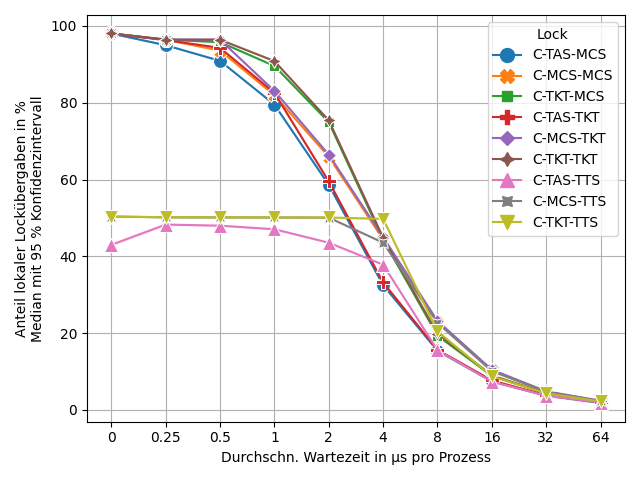
\includegraphics[width=\textwidth]{benchmarks/intelmpi/cohort-mcs-spin-tkt/WBAB-processes=112,mpi_progress=1-local-releases}
        \caption{Anteil lokaler Lockübergaben in \%}
        \label{ben:cohort_mcs_spin_tkt_wbab_112_local_releases}
    \end{subfigure}
    \begin{subfigure}{.5\textwidth}
        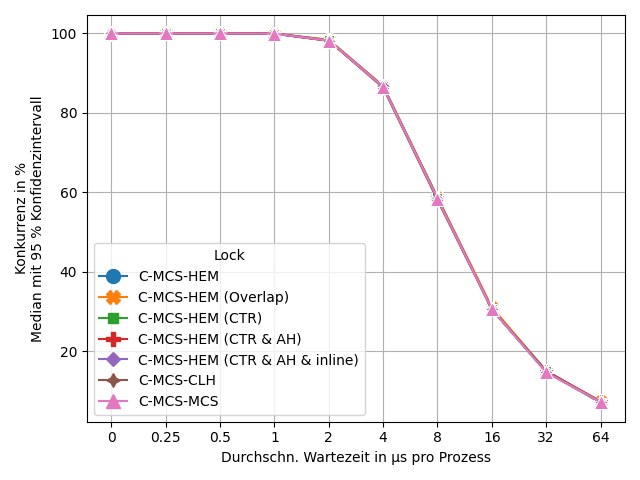
\includegraphics[width=\textwidth]{benchmarks/intelmpi/cohort-mcs-spin-tkt/WBAB-processes=112,mpi_progress=1-global.contention}
        \caption{Globale Konkurrenz in \%}
        \label{ben:cohort_mcs_spin_tkt_wbab_112_global_contention}
    \end{subfigure}
    \begin{subfigure}{.5\textwidth}
        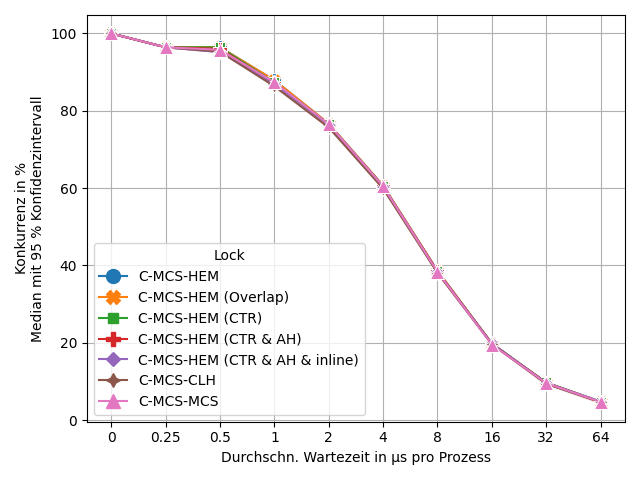
\includegraphics[width=\textwidth]{benchmarks/intelmpi/cohort-mcs-spin-tkt/WBAB-processes=112,mpi_progress=1-local.contention}
        \caption{Lokale Konkurrenz in \%}
        \label{ben:cohort_mcs_spin_tkt_wbab_112_local_contention}
    \end{subfigure}
    \caption{WBAB verschiedener Cohort-Locks mit 112 Prozessen}
    \label{ben:cohort_mcs_spin_tkt_wbab_112}
\end{benchmark}

\autoref{ben:cohort_mcs_spin_tkt_wbab_112} zeigt die Performance der Locks im \gls{wbab}.
\autoref{ben:cohort_mcs_spin_tkt_wbab_112_throughput}
bestätigt die Beobachtungen aus dem \gls{ccwb}:
Ohne Wartezeit gleicht der \gls{wbab} dem \gls{ecsb},
daher sind C-TAS-*-Locks am schnellsten,
sobald aber unkritische Arbeit (in Form von Wartezeit) hinzukommt,
werden sie von den entsprechenden C-MCS-*-Locks überholt.
% Da die unkritische Arbeit im \gls{wbab} niedriger ist als im \gls{ccwb},
% wirkt sich die schlechte Verteilung dieser durch globale \gls{tas}-Locks hier weniger stark aus,
% sodass die C-TKT-*-Locks auch mit Wartezeit am langsamsten bleiben.

Am Overhead in \autoref{ben:cohort_mcs_spin_tkt_wbab_112_overhead} sieht man gut
den wechselnden Einfluss der globalen und lokalen Locks.
Bei geringer Wartezeit (0~\textmu{s} bis 0,5~\textmu{s}) ist wie beim \gls{ecsb}
der lokale Lock ausschlaggebend für die Performance:
Den geringsten Overhead haben die C-*-MCS-Locks,
gefolgt von den C-*-TKT-Locks.
Bei höherer Wartezeit (2~\textmu{s} bis 8~\textmu{s}) hingegen ist wie beim \gls{upb}
der globale Lock entscheidend:
C-MCS-MCS und C-MCS-TKT haben den gleichen Overhead,
ebenso wie C-TAS-MCS und C-TAS-TKT
und auch C-TKT-MCS und C-TKT-TKT.
Die Cohort-Locks mit lokalem \gls{tts}-Lock (C-*-TTS) sind so langsam,
dass dieser Effekt bei ihnen nicht mehr beobachtet werden kann,
bevor die Wartezeit so hoch ist,
dass die Messung ungenau wird.

\autoref{ben:cohort_mcs_spin_tkt_wbab_112_fairness} zeigt,
dass auch im \gls{wbab} die Fairness von C-TAS-*-Locks extrem schlecht ist.
Ohne Wartezeit steigt der Variationskoeffizient auf bis zu 100~\%.
Um das näher zu untersuchen wurde die Konkurrenz seperat für die globalen und lokalen Locks
in den Cohort-Locks gemessen.

Die globale Konkurrenz (vgl. \autoref{ben:cohort_mcs_spin_tkt_wbab_112_global_contention}) zeigt,
dass bei geringer Wartezeit die globalen \gls{tas}-Locks eine sehr geringe Konkurrenz haben,
während diese bei den anderen Locks maximal ist.
Das ist ein klares Indiz dafür,
dass der Lock wiederholt von Prozessen desselben Knotens,
vermutlich des Hauptknotens,
akquiriert wird.
Das erklärt auch die extreme Unfairness.

Bei der lokalen Konkurrenz (vgl. \autoref{ben:cohort_mcs_spin_tkt_wbab_112_local_contention}) ist besonders auffällig,
dass ohne Wartezeit die lokalen \gls{tts}-Locks eine sehr geringe Konkurrenz haben.
Auch hier deutet dies darauf hin,
dass häufig derselbe Prozess mehrmals hinter einander den lokalen Lock akquiriert.
In diesem Fall wirkt sich das aber kaum auf die Fairness aus.
C-MCS-TTS und C-TKT-TTS sind zwar bei einer Wartezeit von 0 unfair,
aber nicht viel unfairer
als bei einer etwas höheren Wartezeit.

Um zu erklären,
warum die Unfairness der C-*-TTS-Locks erst bei einer Wartezeit von 8~\textmu{s} verschwindet,
zeigt \autoref{ben:cohort_mcs_spin_tkt_wbab_112_local_releases} den Anteil der lokalen Lockübergaben,
also wie oft der Cohort-Lock direkt an einen lokalen Nachfolger übergeben wird,
ohne den globalen Lock freizugeben.
Hier wird das Problem dieser Locks deutlich:
Bei einer Wartezeit von unter 8~\textmu{s}
überschreitet der Anteil der lokalen Lockübergaben niemals 50~\%.
Das liegt daran,
dass die Kohortenerkennung im \gls{tts}-Lock bei kurzen kritischen Abschnitten nicht korrekt funktioniert,
wodurch sich lokale und globale Freigaben immer abwechseln.

Um Kohortenerkennung im \gls{tts}-Lock zu ermöglichen,
wurde dieser in \cite{Cohort-Lock} um das \textit{Flag} \textit{successor-exists} erweitert.
Bevor ein Prozess beginnt,
den Lock zu akquirieren,
setzt er dieses \textit{Flag} auf \texttt{true},
um den Anderen zu signalisieren,
dass er auf den Lock wartet.
Sobald der Prozess den Lock akquiriert,
setzt er dieses \textit{Flag} zurück auf \texttt{false}.
Wenn viele Prozesse auf den Lock warten,
würde dieses \textit{Flag} nun fälschlicherweise auf \texttt{false} stehen,
obwohl weitere lokale Nachfolger vorhanden sind.
Daher prüft jeder Prozess in der Warteschleife auch das \textit{successor-exists}-\textit{Flag}
und setzt es auf \texttt{true},
wenn er beobachtet,
dass es zurückgesetzt wurde.

Bei einem sehr kurzen kritischen Abschnitt
haben die anderen Prozesse keine Zeit,
das \textit{successor-exists}-\textit{Flag} zurück auf \texttt{true} zu setzen,
bevor der akquirierende Prozess den Lock wieder freigibt.
Das führt dann zu einer globalen Freigabe.
Der Grund,
weshalb jede zweite Freigabe trotzdem lokal ist,
ist,
dass nach einer globalen Freigabe erst der lokale und anschließend der globale Lock akquiriert wird.
Nachdem ein Prozess den lokalen Lock akquiriert,
muss er also erst auf den globalen Lock warten
und in dieser Zeit können die anderen Prozesse das \textit{successor-exists}-\textit{Flag} zurück auf \texttt{true} setzen.
Das erklärt auch,
warum der C-TAS-TTS-Lock etwas weniger als 50~\% lokale Lockübergaben macht.
Da der globale \gls{tas}-Lock unfair ist,
kann es passieren,
dass ein Prozess ihn freigibt
und der nächste Prozess desselben Knotens ihn direkt wieder akquiriert.
Dieser muss dann nicht auf den globalen Lock warten,
sodass die anderen Prozesse des Knotens
trotz der globalen Freigabe
keine Zeit haben,
das \textit{successor-exists}-\textit{Flag} zurück auf \texttt{true} zu setzen.
In so einem Fall folgt auf eine globale Freigabe keine lokale,
sondern eine weitere globale Freigabe.

Die große Menge an globalen Freigaben
erklärt auch die extrem schlechte Geschwindigkeit der C-*-TTS-Locks
in \autoref{ben:cohort_mcs_spin_tkt_wbab_112_overhead} und \autoref{ben:cohort_mcs_spin_tkt_wbab_112_throughput}.

Insgesamt geht der C-MCS-MCS als Gewinner aus der Evaluation hervor.
Unfaire globale Locks,
wie der \gls{tas}-Lock,
sollten auf verteiltem Speicher vermieden werden,
da diese bei hoher Konkurrenz zu extremer Unfairness führen können,
und lokale \gls{tts}-Locks führen zu extrem schlechter Performance bei kurzen kritischen Abschnitten
und können auch sonst nicht mit den anderen Alternativen mithalten.
Von den verbleibenden vier Cohort-Locks,
bestehend aus MCS- und TKT-Locks,
schneidet der C-MCS-MCS in allen Benchmarks am besten ab
\footnote{%
    Obwohl die Geschwindigkeit des lokalen TKT-Locks durch \hyperref[sec:cohort_opt_3]{Optimierung 3 (Inline Zähler)} verbessert werden kann,
    ändert das nichts an den Ergebnissen der Evaluation:
    Ein lokaler MCS-Lock ist in allen Benchmarks trotzdem schneller (nicht gezeigt).}.

\subsection{Evaluation von lokalen Warteschlangen-Locks}
\label{sec:cohort_hem}

In \autoref{sec:cohort_baseline_evaluation} ist der C-MCS-MCS-Lock als klarer Gewinner hervor gegangen.
Sowohl global als auch lokal verwendet dieser einen Lock mit Warteschlange,
den MCS-Lock.
Dabei ist der MCS-Lock nicht unbedingt der schnellste Warteschlangen-Lock:
In \cite{HCLH-Lock} wird der CLH-Lock als der effizienteste Warteschlangen-Lock
für Rechner mit \gls{Zwischenspeicher}-\gls{Kohaerenz}-Mechanismus bezeichnet
und in den Evaluationen des MCS- und CLH-Locks
in \cite{RH-Lock} und \cite{FC-MCS-Lock}
schneidet der CLH-Lock etwas besser ab
als der MCS-Lock.

Außerdem gibt es einen sehr neuen Warteschlangen-Lock,
den diese Arbeiten noch gar nicht berücksichtigen konnten:
den Hemlock aus \cite{Hemlock}.
Dieser ähnelt sehr dem CLH-Lock,
nutzt aber auch ein paar Techniken aus dem MCS-Lock
und enthält einen ganz neuen Ansatz:
Beim Hemlock gibt es nur einen Warteschlangenknoten pro Prozess für alle Lock-Instanzen.
Dadurch benötigt der Hemlock deutlich weniger Speicher:
Jede zusätzliche Instanz eines Hemlocks benötigt nur einen \texttt{tail}-Zeiger.

Genau wie beim CLH-Lock (vgl. \autoref{fig:clh_init})
enthält ein Warteschlangenknoten des Hemlocks nur ein \texttt{status}-Feld,
auf dessen Änderung ein Nachfolger wartet.
Während beim CLH-Lock höchstens ein Nachfolger auf die Änderung eines \texttt{status}-Feldes wartet,
teilen sich beim Hemlock alle Lock-Instanzen dieselben Warteschlangenknoten.
Bei zwei Hemlock-Instanzen ist es daher möglich,
dass zwei verschiedene Prozesse auf eine Änderung desselben \texttt{status}-Feldes warten,
wenn der Vorgänger der beiden Prozesse beide Lock-Instanzen akquiriert hat.
Aus diesem Grund reicht beim Hemlock kein boolesches \textit{Flag},
wie es im CLH-Lock eingesetzt wird.
Statt einem booleschen \texttt{false}
schreibt ein Vorgänger bei der Freigabe eines Hemlocks die eindeutige Speicheradresse der Lock-Instanz in das \texttt{status}-Feld.
So kann jeder Nachfolger prüfen,
ob die Lockübergabe an ihn gerichtet ist.
Dieser Nachfolger setzt das \texttt{status}-Feld dann zurück auf den speziellen Zeiger \texttt{NULL},
sodass es für die nächste Lockübergabe frei ist.

Wie \autoref{sec:clh_evaluation} gezeigt hat,
eignet sich der CLH-Lock nicht für verteilten Speicher,
da die Prozesse auf eine Änderung im Speicher ihres Vorgängers warten.
Folglich eignet sich der CLH-Lock nicht als globaler Lock im Cohort-Lock.
Dasselbe gilt auch für den Hemlock.
Innerhalb eines Rechenknotens gibt es hingegen gemeinsamen Speicher und \gls{Zwischenspeicher},
daher wird nun evaluiert,
ob sich diese beiden Locks als lokale Locks eignen.

In \cite{Hemlock} werden neben dem Basis-Algorithmus des Hemlocks drei Optimierungen vorgestellt:
Overlap, \textit{Coherence Traffic Reduction} (CTR) und \textit{Aggressive Hand-over} (AH).
Die Overlap-Optimierung wird von den Autoren zwar erläutert,
aber nicht empfohlen,
da sie keine große Verbesserung beobachten konnten.
Der Pseudocode dieser Optimierung hatte in \cite{Hemlock} einen Fehler,
der zu Deadlocks führte
und im Rahmen dieser Masterarbeit aufgefallen ist.
Die Autoren von \cite{Hemlock} wurden darüber informiert
und haben daraufhin eine neue Version (v4) ihrer Arbeit veröffentlicht,
in der der Fehler behoben ist.

Die CTR-Optimierung ist eine geschickte Verwendung von atomaren Operationen,
die zu einer besseren Nutzung der \gls{Zwischenspeicher} führt.
Diese wurde speziell für \gls{Zwischenspeicher}-Cohärenz-Mechanismen vom Typ MESI oder \glstext{mesif} entwickelt.
Dabei steht \glstext{mesif} für \glsdesc{mesif} und bezeichnet die Status,
die ein Speicherbereich im \gls{Zwischenspeicher} haben kann.
Zur Erinnerung:
In dieser Arbeit werden die Benchmarks auf Intels Haswell Prozessoren ausgeführt.
Diese nutzen einen auf \glstext{mesif} basierenden Mechanismus \cite{Haswell-cache-coherence}.
Damit ist eine Betrachtung dieser Optimierung sinnvoll.

Durch die AH-Optimierung wird die Lockübergabe spekulativ ausgeführt,
bevor geprüft wird,
ob es überhaupt einen Nachfolger gibt.
Dadurch wird der kritische Pfad bei Konkurrenz kürzer,
was den Lock schneller macht.
So eine spekulative Lockübergabe hat aber auch einen Nachteil:
Abhängig von der Speicherverwaltung kann es
durch \textit{use-after-free}-Fehler
zum Programmabsturz kommen \cite{Hemlock}.
Bei der Nutzung von \gls{mpi} wird der gemeinsame Speicher über ein \gls{Fenster} verwaltet.
Da ein \gls{Fenster} von allen beteiligten Prozessen freigegeben werden muss,
bevor der Speicher selbst freigegeben wird,
können solche \textit{use-after-free}-Fehler hier nicht auftreten.
In \cite{Hemlock} werden noch zwei Varianten der AH-Optimierung vorgestellt,
die solche Fehler vermeiden.
Jedoch schreiben die Autoren,
dass der Hemlock mit CTR und AH die beste Performance hat
und daher zu bevorzugen ist,
wenn die Speicherverwaltung es zulässt.
Aus diesem Grund werden die beiden Varianten der AH-Optimierung in dieser Arbeit nicht untersucht.

\begin{benchmark}[h]
    \begin{subfigure}{.5\textwidth}
        \includegraphics[width=\textwidth]{benchmarks/intelmpi/cohort-hem/CCWB-processes=28-latency}
        \caption{Iterationsdauer in \textmu{s}}
        \label{ben:cohort_hem_ccwb_28_latency}
    \end{subfigure}
    \begin{subfigure}{.5\textwidth}
        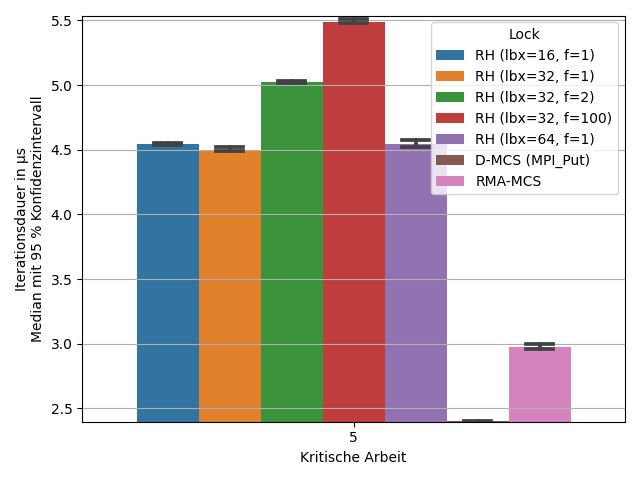
\includegraphics[width=\textwidth]{benchmarks/intelmpi/cohort-hem/CCWB-processes=28-latency-max}
        \caption{Iterationsdauer in \textmu{s}}
        \label{ben:cohort_hem_ccwb_28_latency_max}
    \end{subfigure}
    \caption{CCWB von C-MCS-HEM mit 28 Prozessen}
    \label{ben:cohort_hem_ccwb_28}
\end{benchmark}

\autoref{ben:cohort_hem_ccwb_28_latency} zeigt die Geschwindigkeit der Cohort-Locks mit den lokalen Hemlock-Varianten
und einem lokalen CLH-Lock
im Vergleich zum C-MCS-MCS-Lock.
Für den Benchmark wurde nur ein Rechenknoten verwendet (daher 28 Prozesse),
damit der Overhead des globalen Locks geringer ist
und die Unterschiede zwischen den verschiedenen lokalen Locks stärker hervortreten.
In \autoref{ben:cohort_hem_ccwb_28_latency_max} ist eine Nachaufnahme der Geschwindigkeiten
bei einer kritischen Arbeit von 5 zu sehen.
In dieser sieht man die Unterschiede noch besser.
Die Fairness wird nicht gezeigt.
Da alle Locks \gls{fifo}-Warteschlangen nutzen,
sind alle sehr fair.

In diesem Benchmark ist der lokale CLH-Lock langsamer
als der lokale MCS-Lock.
Die Overlap-Optimierung des Hemlocks führt,
wie in \cite{Hemlock} beschrieben,
nicht zu einer Verbesserung.
CTR,
insbesondere in Kombination mit AH,
hingegen schon.
Trotzdem ist der C-MCS-HEM mit CTR und AH deutlich langsamer
als die Cohort-Locks mit lokalem CLH- und MCS-Lock.

Der Grund dafür ist \hyperref[sec:cohort_opt_3]{Optimierung 3 (Inline Zähler)} des Cohort-Locks aus \autoref{sec:cohort_opt_3},
die auf den lokalen CLH- und MCS-Lock,
aber nicht auf den Hemlock angewandt wurde.
Genau wie der TKT-Lock nutzt auch der Hemlock kein boolesches \textit{Flag} für die Lockübergabe.
Daher wurde in dieser Arbeit auch der lokale Hemlock um ein Feld erweitert,
mit dem die Anzahl der lokalen Lockübergaben an den Nachfolger kommuniziert wird.

Um den Hemlock besser mit dem CLH- und MCS-Lock vergleichen zu können,
wurde dieser angepasst,
sodass ein Nachfolger nicht auf die eindeutige Speicheradresse des Locks,
sondern,
wie bei den beiden anderen Locks,
auf einen booleschen Wert wartet.
Durch diese Anpassung konnte auch auf den Hemlock \hyperref[sec:cohort_opt_3]{Optimierung 3} angewandt werden,
aber die Warteschlangenknoten können nicht mehr von mehreren Prozessen verwendet werden.
Der Hemlock hat also keinen Vorteil mehr im Bezug auf Speicherverbrauch.
Das könnte jedoch leicht behoben werden,
indem der Zähler für lokale Lockübergaben und die eindeutige Speicheradresse des Locks
(oder eine andere Zahl, die die Lock-Instanz eindeutig identifiziert)
in einen gemeinsamen Speicherbereich kodiert werden
(vgl. Diskussion über \hyperref[sec:cohort_opt_3]{Optimierung 3} für TKT-Lock).
Da der Speicherverbrauch in dieser Arbeit nicht untersucht wird,
wurde auf so eine Kodierung verzichtet.

In \autoref{ben:cohort_hem_ccwb_28_latency_max} sieht man deutlich die Verbesserung durch \hyperref[sec:cohort_opt_3]{Optimierung 3}.
Der angepasste Hemlock überholt sogar den lokalen MCS-Lock,
obwohl er wie der CLH-Lock \gls{numa} nicht optimal nutzen kann.
Mit diesen Optimierungen setzt sich der C-MCS-HEM knapp als schnellster Lock im \gls{ccwb} durch.

\begin{benchmark}[h]
    \begin{subfigure}{.5\textwidth}
        \includegraphics[width=\textwidth]{benchmarks/intelmpi/cohort-hem/WBAB-processes=112,mpi_progress=1-overhead}
        \caption{Iterationsdauer in \textmu{s}}
        \label{ben:cohort_hem_wbab_112_overhead}
    \end{subfigure}
    \begin{subfigure}{.5\textwidth}
        \includegraphics[width=\textwidth]{benchmarks/intelmpi/cohort-hem/WBAB-processes=112,mpi_progress=1-throughput}
        \caption{Durchsatz in Mio/s}
        \label{ben:cohort_hem_wbab_112_throughput}
    \end{subfigure}
    \caption{WBAB von C-MCS-HEM mit 112 Prozessen}
    \label{ben:cohort_hem_wbab_112}
\end{benchmark}

Um die Performance auf mehreren Rechenknoten zu evaluieren,
zeigt \autoref{ben:cohort_hem_wbab_112} die Ergebnisse des \gls{wbab}
mit 112 Prozessen,
also vier Rechenknoten.
Diese Ergebnisse unterscheiden sich kaum
von denen des \gls{wbab}s mit nur einem Rechenknoten (nicht gezeigt).
Der \gls{ccwb} mit 112 Prozessen wird nicht gezeigt,
da die Konfidenzintervalle durch die vielen entfernten Zugriffe des Benchmarks so ungenau sind,
dass die Locks nicht aussagekräftig miteinander verglichen werden können.

\autoref{ben:cohort_hem_wbab_112_overhead} und \autoref{ben:cohort_hem_wbab_112_throughput} zeigen,
dass auch im \gls{wbab} die Overlap-Optimier-ung keine Verbesserung bringt,
während der Hemlock mit CTR etwas schneller
und mit zusätzlich AH deutlich schneller wird.
Wie bereits im \gls{ccwb} mit 28 Prozessen (vgl. \autoref{ben:cohort_hem_ccwb_28}) überholt der Hemlock aber erst mit Nutzung von \hyperref[sec:cohort_opt_3]{Optimierung 3 (Inline Zähler)}
den CLH-Lock.
Ohne Wartezeit bleibt in diesem Benchmark der C-MCS-MCS-Lock der schnellste Lock,
bei einer Wartezeit von 0,25~\textmu{s} wird er aber knapp vom C-MCS-CLH-Lock und dem voll optimierten C-MCS-HEM-Lock überholt.
Danach ist zwischen den drei Locks kein Unterschied mehr zu erkennen.

Zusammenfassend lässt sich sagen,
dass ein Cohort-Lock mit lokalem Hemlock eine sehr gute Performance hat.
In den meisten Fällen ist er genauso schnell
wie ein Cohort-Lock mit lokalem MCS-Lock,
in manchen Fällen etwas schneller
und in manchen Fällen etwas langsamer.
Dabei benötigt er aber deutlich weniger Speicherplatz,
da mehrere Lock-Instanzen dieselben Warteschlangenknoten verwenden können.
Das ist ein klarer Vorteil.

\section{AHMCS-Lock}
\label{sec:ahmcs-lock}

Der adaptive HMCS-Lock (kurz AHMCS-Lock) aus \cite{AHMCS-Lock} basiert auf dem HMCS-Lock aus \cite{HMCS-Lock}.
Wie bereits in \autoref{sec:cohort-lock} erklärt,
ist ein HMCS-Lock eine optimierte Verallgemeinerung eines Cohort-Locks für beliebig viele Hierarchieebenen,
wobei auf jeder Ebene ein MCS-Lock verwendet wird.
Das hat zwar den Vorteil,
dass bei hoher \gls{Konkurrenz} die Lokalität auf jeder Ebene,
z.~B. durch L1-, L2- und L3-\gls{Zwischenspeicher},
perfekt genutzt werden kann.
Es führt jedoch bei geringer \gls{Konkurrenz} zu mehr Overhead,
da Prozesse dann mehrere Locks akquirieren müssen.
Bei einem freien HMCS-Lock muss ein Prozess sogar die Locks aller Hierarchieebenen nacheinander akquirieren.

Der AHMCS-Lock vermeidet dieses Problem,
indem er Prozessen erlaubt,
direkt die Locks der höheren Ebenen zu akquirieren,
ohne die Locks der unteren Ebenen zu besitzen.
Die Einstiegsebene wird dabei abhängig von der \gls{Konkurrenz} durch Hysterese bestimmt.
D.~h., jeder Prozess misst die \gls{Konkurrenz} bei Akquirieren und Freigeben des Locks
und entscheidet darauf basierend,
auf welcher Ebene er beim nächsten Mal mit der Akquisition beginnen soll.
Um die \gls{Konkurrenz} zu messen,
beobachtet der Prozess,
ob er auf seiner Einstiegsebene einen Vorgänger
und ob er einen Nachfolger hat.
Wenn beides der Fall ist,
wird eine hohe \gls{Konkurrenz} angenommen
und der Prozess steigt beim nächsten Mal eine Ebene niedriger ein.
Wird weder ein Vorgänger,
noch ein Nachfolger beobachtet,
wird eine niedrige \gls{Konkurrenz} angenommen
und der Prozess steigt beim nächsten Mal eine Ebene höher ein.
Ansonsten nutzt der Prozess auch beim nächsten Mal wieder dieselbe Einstiegsebene.

So passt sich der AHMCS-Lock dynamisch an die Konkurrenzsituation an.
Wenn keine \gls{Konkurrenz} vorliegt,
nutzen Prozesse bei jedem Mal eine höhere Ebene,
wodurch sich der HMCS-Lock nach ein paar Akquisitionen wie ein normaler MCS-Lock verhält,
da alle Prozesse direkt den globalen MCS-Lock akquirieren.
Liegt hingegen eine hohe \gls{Konkurrenz} vor,
wandern Prozesse in der Hierarchie immer weiter nach unten,
wodurch der AHMCS-Lock sich wie ein HMCS-Lock verhält
und die Lokalität auf jeder Ebene nutzt.

Wenn nach einer gewissen Zeit von hoher \gls{Konkurrenz}
die \gls{Konkurrenz} plötzlich stark abfällt,
braucht die Anpassung der Einstiegsebenen durch Hysterese einige Akquisitionen.
Um bei so einem Szenario schneller reagieren zu können,
ist in den AHMCS-Lock eine Abkürzung eingebaut.
Jeder Prozess prüft als Erstes,
ob der Lock auf seiner Einstiegsebene frei ist
und wenn ja,
ob auch der globale MCS-Lock frei ist.
Ist beides der Fall,
akquiriert er den globalen Lock direkt
und überspringt alle unteren Ebenen.
Erst wenn wieder \gls{Konkurrenz} vorliegt,
wird die Einstiegsebene wieder durch Hysterese angepasst.

Wenn ein System \gls{htm} unterstützt,
kann diese Abkürzung noch effizienter implementiert werden.
\Gls{htm} erlaubt es,
Transaktionen mit Hardwareunterstützung auszuführen.
Dabei ist garantiert,
dass der gesamte Code innerhalb einer Transaktion atomar ausgeführt wird.
Wird ein Konflikt mit der Transaktion eines anderen Prozesses festgestellt,
wird die Transaktion abgebrochen und alle Änderungen rückgängig gemacht.
\gls{htm} wird in \cite{AHMCS-Lock} genutzt,
um den kritischen Abschnitt spekulativ auszuführen,
statt den globalen MCS-Lock zu akquirieren,
wenn die Abkürzung verwendet wird.
Bricht die Transaktion ab,
fällt der Prozess auf den normalen Weg mit Hysterese zurück.

In dieser Arbeit werden,
wie in \autoref{sec:cohort-lock} erläutert,
nur Locks mit zwei Hierarchieebenen betrachtet.
Eine Hysterese ist aber erst bei einer höheren Anzahl an Ebenen von Nutzen.
Der \gls{upb} hat in \autoref{ben:baseline_upb} bereits gezeigt,
dass der Geschwindigkeitsunterschied zwischen dem D-MCS mit einer Ebene und dem RMA-MCS mit zwei Ebenen gering ist,
wenn die Locks frei sind,
und es viel wichtiger ist \gls{rma}-Zugriffe,
besonders auf entfernten Speicher,
zu vermeiden.

Auch die Abkürzung bringt bei nur zwei Hierarchieebenen keinen Vorteil,
da immer der lokale und globale Lock überprüft werden,
um Ebenen zu überspringen.
Ein normaler Cohort-Lock hat aber keine weiteren Ebenen,
neben dem lokalen und globalen Lock.
Und auch \gls{htm} kann im Rahmen dieser Arbeit nicht genutzt werden,
da das CoolMUC-2 Linux Cluster des \gls{lrz} \gls{htm} nicht unterstützt.

Aus diesen Gründen ist es nicht sinnvoll,
den AHMCS-Lock auf verteilten Speicher zu portieren.
Auf einem System mit \gls{htm}-Support,
oder wenn der Lock z.~B. nur mit Open-MPI funktionieren muss,
sodass mehrere Hierarchieebenen unterstützt werden können,
könnte sich dieser Lock im Rahmen einer anderen Arbeit aber als nützlich erweisen.

\clearpage

\section{CST-Lock}
\label{sec:cst-lock}

Der CST-Lock \cite{CST-Lock} basiert auf einem Cohort-Lock \cite{Cohort-Lock}
mit einem globalen MCS-Lock \cite{MCS-Lock} und einem lokalen K42-Lock \cite{K42-Lock} (einer Variante des MCS-Locks)
und hat im wesentlichen zwei große Verbesserungen:
\begin{enumerate}
    \item Der benötigte Speicher wird möglichst spät dynamisch allokiert,
          sodass kein unnötiger Speicher für Prozesse verbraucht wird,
          die den Lock vielleicht gar nicht nutzen.
          Das ist in Systemen mit gemeinsamem Speicher sinnvoll,
          da vorher nicht klar ist,
          welche Prozesse den Lock nutzen.
    \item Der Scheduler wird berücksichtigt,
          d.~h., Prozesse warten nur so lange aktiv,
          bis die ihnen vom Scheduler zugeteilte Zeitscheibe abläuft
          und werden dann geparkt,
          bis sie von ihrem Vorgänger aufgeweckt werden.
          Das sorgt für eine bessere Performance bei überladenen Systemen,
          die mehr Prozesse ausführen,
          als Prozessoren zur Verfügung stehen,
          da wartende Prozesse nach Ablauf ihrer Zeitscheibe keinen Prozessor mehr blockieren.
\end{enumerate}
Diese beiden Verbesserungen sind aber bei verteilten Systemen im Bereich \gls{hpc} nicht so relevant,
da erstens alle Prozesse,
die den Lock nutzen möchten,
ein gemeinsames \gls{Fenster} erzeugen müssen,
d.~h. wenn bekannt ist,
dass manche Prozesse den Lock nicht benötigen,
können diese ausgeschlossen werden
und zweitens im \gls{hpc}-Bereich Systeme typischerweise nicht überladen sind,
da für optimale Performance in der Regel genau so viele Prozessoren verwendet,
wie Prozesse ausgeführt werden.
Der CST-Lock ist daher kein guter Kandidat für eine Portierung auf verteilten Speicher.

\section{SHFL-Lock}
\label{sec:shfl-lock}

Der SHFL-Lock aus \cite{Shfl-Lock}
kombiniert einen \gls{tts}-Lock (siehe \autoref{sec:spin_locks})
mit einem MCS-Lock (siehe \autoref{sec:mcs_lock}):
Ein Prozess versucht erst einmalig,
den \gls{tts}-Lock zu akquirieren.
Wenn er das nicht schafft,
akquiriert er den MCS-
und dann den \gls{tts}-Lock.
Durch den MCS-Lock ist sichergestellt,
dass bei hoher Konkurrenz nicht alle Prozesse ständig
über den \gls{tts}-Lock
auf denselben Speicherbereich zugreifen
und durch den \gls{tts}-Lock können Prozesse bei geringer Konkurrenz
den Overhead des MCS-Locks vermeiden.

Das Besondere beim SHFL-Lock ist,
dass die Reihenfolge der Warteschlangenknoten des MCS-Locks
während des Wartens
geändert wird.
Diese werden gruppiert,
sodass Prozesse desselben \gls{numa}-Knotens in der Schlange beieinanderliegen
und aufeinanderfolgend den kritischen Abschnitt betreten.
Die Sortierung der Warteschlange wird dabei zunächst von dem Prozess durchgeführt,
der bereits den MCS-Lock akquiriert hat,
aber noch auf den \gls{tts}-Lock wartet.
Dieser Prozess iteriert durch die Schlange
und bewegt die Knoten aller Prozesse,
die auch auf seinem \gls{numa}-Knoten laufen,
an den Anfang der Schlange.
Den letzten Prozess,
dessen Knoten er bewegt hat,
ernennt er dann zum neuen Sortierer.

Durch diese Strategie wird die Sortierung der Warteschlange von den Prozessen ausgeführt,
die sonst sowieso nur warten würden.
Da immer nur ein Prozess gleichzeitig sortiert,
muss beim Sortierungsalgorithmus nicht auf \textit{race conditions} geachtet werden.
Lediglich der letzte Knoten der Warteschlange darf nicht bewegt werden,
da sich hier nebenläufig weitere Prozesse einreihen können.

\begin{figure}[h]
    \centering
    \begin{tabular}{c}\begin{lstlisting}
if (tts_lock.disabled_and_locked.load() == {0, 0})
  if (tts_lock.disabled_and_locked.cas({0, 0}, {0, 1}))
    return; // Lock geklaut

bool first = mcs_lock.acquire();
if (first) // Deaktiviere Klauen
  tts_lock.disabled.store(1);

do {
  if (mcs_node.batch == 0 || mcs_node.is_shuffler)
    shuffle_waiters();
  while (tts_lock.locked.load() == 1);
} while (!tts_lock.locked.cas(0, 1));

bool last = mcs_lock.release();
if (last) // Aktiviere Klauen
  tts_lock.disabled.store(0);
    \end{lstlisting}\end{tabular}
    \caption{Akquirieren eines SHFL-Locks (\texttt{acquire})}
    \label{fig:shfl_acquire}
\end{figure}

\autoref{fig:shfl_acquire} zeigt eine vereinfachte C++-Implementierung der Akquisition.
Wenn ein Prozess direkt in Zeile 1-3 den \gls{tts}-Lock akquiriert,
ohne den MCS-Lock zu nutzen,
spricht man davon,
dass der Prozess den Lock klaut.
Um zu verhindern,
dass ein neuer Prozess alle wartenden Prozesse überholt,
indem er den Lock klaut,
obwohl bereits ein Prozess den MCS-Lock akquiriert hat
und in Zeile 9-13 auf den \gls{tts}-Lock wartet,
ist der \gls{tts}-Lock so modifiziert,
dass das Klauen deaktiviert werden kann.
Dafür nutzt er zwei Bytes:
Das \texttt{locked}-Byte enthält die Information,
ob er bereits akquiriert ist
und das \texttt{disabled}-Byte enthält die Information,
ob er deaktiviert ist.
Um den SHFL-Lock zu klauen,
darf der \gls{tts}-Lock weder deaktiviert,
noch akquiriert sein.
Dies wird sichergestellt,
indem \texttt{disabled} und \texttt{locked} gemeinsam
mit einer \gls{cas}-Operation atomar
von \texttt{\{0, 0\}} auf \texttt{\{0, 1\}} geändert werden
(siehe \autoref{fig:shfl_acquire}, Zeile 2).
Wenn nicht beide Bytes 0 sind,
schlägt die \gls{cas}-Operation fehl
und der Prozess fährt fort,
indem er den MCS-Lock akquiriert.

Der MCS-Lock,
den der SHFL-Lock nutzt,
ist ebenfalls modifiziert:
Die \texttt{acquire}-Funktion liefert \texttt{true} zurück,
wenn der Prozess nicht auf einen Vorgänger warten musste,
sondern den MCS-Lock direkt akquirieren konnte.
In diesem Fall deaktiviert er den \gls{tts}-Lock in Zeile 7,
sodass der Lock nicht mehr geklaut werden kann,
bis die Warteschlange wieder leer ist.

Nachdem der Prozess den MCS-Lock akquiriert hat,
prüft er in Zeile 10,
ob er für die Sortierung verantworlich ist
und führt diese ggf. durch.
Anschließend wartet er in Zeile 12 auf den \gls{tts}-Lock
und versucht ihn in Zeile 13 mit einer \gls{cas}-Operation zu akquirieren.
Wenn das fehlschlägt,
sortiert er die Warteschlange ggf. erneut.
Im Gegensatz zu Zeile 1 und 2
wird in Zeile 12 und 13 das \texttt{disabled}-Byte ignoriert.
Der \gls{tts}-Lock kann hier also auch dann akquiriert werden,
wenn das Klauen deaktiviert ist.

Für die Sortierung iteriert der Prozess über die Warteschlange
und verschiebt jeden Knoten,
dessen Prozess auf demselben \gls{numa}-Knoten läuft,
hinter den Knoten,
den er zuletzt verschoben hat.
Den ersten gefunden Knoten verschiebt er hinter seinen eigenen Knoten.
Dabei benutzt er das Feld \texttt{batch},
um alle verschobenen Knoten (inklusive seines eigenen Knotens) zu nummerieren.
Die Nummerierung beginnt mit der Zahl 1.
Nachdem der Sortierer einmal über die Warteschlange iteriert ist,
sind alle Knoten desselben \gls{numa}-Knotens an den Anfang der Warteschlange verschoben worden
und haben aufsteigende Werte in ihrem \texttt{batch}-Zähler.
Der Sortierer setzt dann das \textit{Flag} \texttt{is\_shuffler}
des letzten verschobenen Knotens
auf \texttt{true}
und beendet seine Sortierung.

Für die Prüfung,
ob der Prozess die Warteschlangen sortieren soll,
gibt es daher zwei Kriterien:
Wenn in Zeile 10 sein \texttt{batch}-Zähler noch den Initialwert 0 hat,
ist er der erste Sortierer seines \gls{numa}-Knotens.
Ist hingegen sein \texttt{is\_shuffler}-\textit{Flag} \texttt{true},
so wurde er von einem Vorgänger zum Sortierer ernannt.
In beiden Fällen soll er die Warteschlange sortieren.

Um zu verhindern,
dass immer die Prozesse eines \gls{numa}-Knotens an den Anfang der Warteschlange verschoben werden
und andere Prozesse \glslink{Verhungern}{verhungern},
wird der \texttt{batch}-Zähler zu Beginn jeder Sortierung überprüft.
Wenn er einen Schwellwert überschreitet,
wird die Sortierung abgebrochen,
sodass nach einer Weile
der nächste Knoten mit einem \texttt{batch}-Wert von 0
den MCS-Lock akquiriert
und zum neuen Sortierer wird.

Da ein ganzer Sortierungslauf zu lange dauern könnte,
prüft der Sortierer außerdem am Ende jeder Iteration,
ob der \gls{tts}-Lock inzwischen frei ist,
bevor er mit dem nächsten Knoten fortfährt.
Ist das der Fall,
ernennt er ebenfalls den Prozess des letzten verschobenen Knotens zum neuen Sortierer
und beendet seine Sortierung vorzeitig.

Durch das \texttt{is\_shuffler}-\textit{Flag} kann es passieren,
dass ein Prozess zum Sortierer ernannt wird,
der gerade auf den MCS-Lock wartet.
Daher ist der MCS-Lock zusätzlich so modifiziert,
dass wartende Prozesse immer wieder ihr \texttt{is\_shuffler}-\textit{Flag} prüfen
und ggf. auch die Funktion \texttt{shuffle\_waiters} aufrufen.
In diesem Fall prüft der Sortierer am Ende jeder Iteration allerdings,
ob der MCS-Lock inzwischen frei ist,
nicht der \gls{tts}-Lock.

Nachdem ein Prozess ggf. die Warteschlange sortiert
und den \gls{tts}-Lock akquiriert hat,
gibt er den MCS-Lock in Zeile 15 direkt wieder frei.
Wenn er dabei der letzte Prozess in der Warteschlange war,
aktiviert er in Zeile 17 wieder die Möglichkeit den SHFL-Lock zu klauen.

Der kritische Abschnitt wird eigentlich nur durch den \gls{tts}-Lock geschützt,
der MCS-Lock dient lediglich dazu,
eine hohe Konkurrenz auf dem \gls{tts}-Lock zu vermeiden
und eine Warteschlange zu haben,
die sortiert werden kann,
um lokale Nachfolger zu bevorzugen.
Um den SHFL-Lock freizugeben,
muss daher nach dem Ausführen des kritischen Abschnitts
nur noch der \gls{tts}-Lock freigegeben werden
(siehe \autoref{fig:shfl_release}).

\begin{figure}[h]
    \centering
    \begin{tabular}{c}\begin{lstlisting}
tts_lock.locked.store(0);
    \end{lstlisting}\end{tabular}
    \caption{Freigeben eines SHFL-Locks (\texttt{release})}
    \label{fig:shfl_release}
\end{figure}

\subsection{Portierung und Optimierung des SHFL-Locks}

Bei der Portierung auf verteilen Speicher
wurde eine kleine Optimierung
in der nicht gezeigten Funktion \texttt{shuffle\_waiters} durchgeführt.
In \cite{Shfl-Lock} wird in jeder Iteration
sowohl für den betrachteten Knoten,
als auch für dessen Vorgänger geladen,
zu welchem \gls{numa}-Knoten er gehört.
Das ist kein Problem auf Systemen mit gemeinsamem Speicher,
da der Wert beim ersten Zugriff in den \gls{Zwischenspeicher} geladen wird.
Auf verteiltem Speicher führt solcher Code hingegen zu unnötig vielen entfernten Zugriffen.
Die portierte Version speichert daher den Wert des aktuellen Knotens in einer lokalen Variable
und verwendet diese in der nächsten Iteration wieder,
statt den Wert neu zu laden.

Ein großes Problem des SHFL-Locks auf verteiltem Speicher
ist die Verwendung eines \gls{tts}-Locks.
Während \gls{tts}-Locks auf gemeinsamem Speicher schneller sind
als \gls{tas}-Locks,
ist das auf verteiltem Speicher genau umgekehrt,
da ein \gls{tts}-Locks deutlich mehr entfernte Zugriffe benötigt.
Daher wird auch eine Variante des SHFL-Locks evaluiert,
in der der \gls{tts}-Lock durch einen \gls{tas}-Lock ersetzt ist.
Dafür müssen in \autoref{fig:shfl_acquire} lediglich Zeile 1 und 12 entfernt werden.

\subsection{Evaluation des SHFL-Locks}

Für die Evaluation werden der portierte SHFL-Lock
und die SHFL-Lock-Variante mit \gls{tas}-Lock
mit dem optimierten MCS-Lock
basierend auf D-MCS aus \autoref{sec:optimierung_dmcs} verglichen.
Um den Effekt der Sortierung zu untersuchen,
wird zusätzlich noch eine Kombination aus \gls{tts}- und MCS-Lock evaluiert,
die dem SHFL-Lock entspricht,
aber die Reihenfolge der Warteschlange unverändert lässt
(\autoref{fig:shfl_acquire} ohne Zeile 10 und 11),
sowie eine entsprechende Kombination aus \gls{tas}- und MCS-Lock
(\autoref{fig:shfl_acquire} ohne Zeile 1 und 10-12).

\begin{benchmark}[!h]
    \begin{subfigure}{.5\textwidth}
        \includegraphics[width=\textwidth]{benchmarks/intelmpi/shfl/UPB-lock_count=1000-latency}
        \caption{UPB}
        \label{ben:shfl_upb}
    \end{subfigure}
    \begin{subfigure}{.5\textwidth}
        \includegraphics[width=\textwidth]{benchmarks/intelmpi/shfl/ECSB-latency}
        \caption{ECSB}
        \label{ben:shfl_ecsb}
    \end{subfigure}
    \begin{subfigure}{.5\textwidth}
        \includegraphics[width=\textwidth]{benchmarks/intelmpi/shfl/CCWB-processes=28-latency}
        \caption{CCWB mit 28 Prozessen}
        \label{ben:shfl_ccwb_28}
    \end{subfigure}
    \begin{subfigure}{.5\textwidth}
        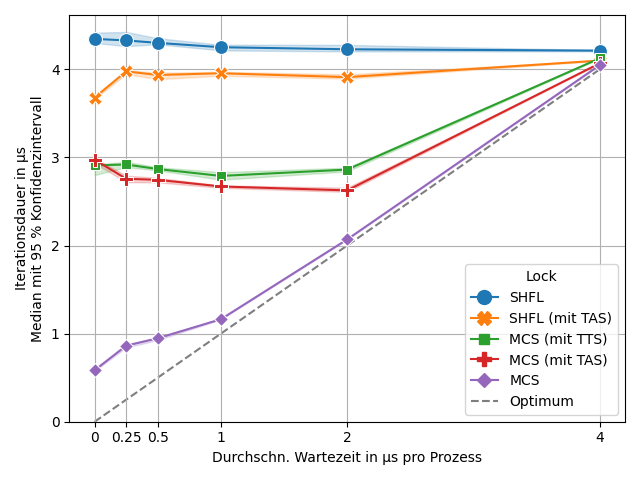
\includegraphics[width=\textwidth]{benchmarks/intelmpi/shfl/WBAB-processes=28,mpi_progress=1-latency}
        \caption{WBAB mit 28 Prozessen}
        \label{ben:shfl_wbab_28}
    \end{subfigure}
    \begin{subfigure}{.5\textwidth}
        \includegraphics[width=\textwidth]{benchmarks/intelmpi/shfl/CCWB-processes=112-latency}
        \caption{CCWB mit 112 Prozessen}
        \label{ben:shfl_ccwb_112}
    \end{subfigure}
    \begin{subfigure}{.5\textwidth}
        \includegraphics[width=\textwidth]{benchmarks/intelmpi/shfl/WBAB-processes=112,mpi_progress=1-latency}
        \caption{WBAB mit 112 Prozessen}
        \label{ben:shfl_wbab_112}
    \end{subfigure}
    \caption{Iterationsdauer in \textmu{s} des Shfl-Locks in allen Benchmarks}
    \label{ben:shfl}
\end{benchmark}

\autoref{ben:shfl_upb} zeigt die Geschwindigkeit im \gls{upb}:
Auf dem Hauptknoten sind alle Locks ziemlich schnell,
da durch die Möglichkeit,
den Lock zu klauen,
nur ein freier \gls{tts}- oder \gls{tas}-Lock akquiriert werden muss.
Man sieht allerdings,
dass die Varianten mit \gls{tts}-Lock etwas langsamer sind.
Wenn der akquirierende Prozess auf einem anderen Knoten läuft,
gibt es denselben Unterschied.
Dieser ist aber um ein Vielfaches ausgeprägter,
da es sich nun um entfernte Speicherzugriffe handelt.

Bei geringer Konkurrenz ist ein \gls{tas}-Lock schneller
als ein \gls{tts}-Lock,
da letzterer zusätzliche unnötige lesende Zugriffe ausführt.
Im SHFL-Lock wird die Konkurrenz um den \gls{tts}-Lock
durch den MCS-Lock gering gehalten.
Daher liegt es nahe,
das auch auf gemeinsamem Speicher
(hier sind \gls{tts}-Locks bei hoher Konkurrenz schneller),
ein SHFL-Lock mit \gls{tas}-Lock in jeder Konkurrenzsituation schneller ist
als ein SHFL-Lock mit \gls{tts}-Lock.
Dies wird durch \autoref{ben:shfl_ccwb_28} und \autoref{ben:shfl_wbab_28} bestätigt.

Im Gegensatz zum \gls{upb} zeigt der \gls{ecsb} in \autoref{ben:shfl_ecsb} Unterschiede zwischen allen Locks:
Der SHFL-Lock ist hier extrem langsam
mit einer Iterationsdauer von bis zu 30~\textmu{s},
gefolgt von der Variante mit \gls{tas}-Lock
mit bis zu 25~\textmu{s} Iterationsdauer.
Auch die Kombination von \gls{tts}- bzw. \gls{tas}- und MCS-Lock ist sehr langsam
mit einer Iterationsdauer von bis zu 18~\textmu{s} bzw. 13~\textmu{s}.
Der reine MCS-Lock hat zum Vergleich eine Iterationsdauer von unter 5~\textmu{s}
und ist damit in diesem Benchmark mehr als sechs Mal so schnell
wie der SHFL-Lock.
Der \gls{ccwb} in \autoref{ben:shfl_ccwb_112}
und der \gls{wbab} in \autoref{ben:shfl_wbab_112} zeigen ein ähnliches Bild.

Die beiden Besonderheiten des SHFL-Locks,
zum einen die Kombination von \gls{tts}- und MCS-Lock für die Möglichkeit,
den Lock zu klauen
und zum anderen die Sortierung der Warteschlange,
führen also beide auf verteiltem Speicher zu einer Verschlechterung der Geschwindigkeit,
selbst wenn statt einem \gls{tts}- ein \gls{tas}-Lock verwendet wird:
In allen Benchmarks,
außer dem \gls{upb},
ist die Kombination von \gls{tas}- und MCS-Lock deutlich langsamer
als ein reiner MCS-Lock.
Der SHFL-Lock,
welcher zusätzlich die Warteschlange sortiert,
ist noch einmal deutlich langsamer.

Während auf gemeinsamem Speicher \textit{Spin}-Locks,
wie der \gls{tts}- und \gls{tas}-Lock,
sehr schnell sind
-- bei geringer Konkurrenz auch schneller als der MCS-Lock --
ist das auf verteiltem Speicher nicht der Fall.
Durch die Abwesenheit eines \gls{Zwischenspeicher}s sind hier viele langsame Zugriffe
auf entfernten Speicher notwendig,
wodurch ein wartender Prozess mit deutlich geringerer Frequenz den Status
des Locks abfragen kann.
Da im SHFL-Lock ein Prozess immer als letztes einen \textit{Spin}-Lock akquirieren muss,
bevor er den kritischen Abschnitt betreten darf,
hängt die Performance des Shfl-Locks stark von diesem \textit{Spin}-Lock ab.
Das ist auf gemeinsamem Speicher gut
und auf verteiltem Speicher schlecht.

Möglicherweise wäre es besser,
zwei MCS-Locks zu kombinieren
oder eine Variante zu finden,
bei der ein Prozess im MCS-Lock effizient feststellen kann,
dass er am Anfang der Warteschlange ist,
sodass er die Sortierung starten kann.
Beides erfordert allerdings eine umfangreiche Anpassung des SHFL-Locks
und ist daher nicht mehr Teil dieser Arbeit.

Selbst wenn man eine Variante findet,
zwei Locks effizient zu kombinieren,
bleibt das Problem,
dass eine Sortierung der Warteschlange die Geschwindigkeit verschlechtert,
statt sie zu verbessern.
Obwohl die Sortierung von Prozessen ausgeführt wird,
die eigentlich nur warten sollten,
wirkt sie sich negativ auf die Geschwindigkeit aus.
Durch die vielen entfernten Zugriffe,
die beim Iterieren über die Warteschlange notwendig sind,
ist eine Iteration auf verteiltem Speicher deutlich langsamer
als auf gemeinsamem Speicher.
Da auf jedem \gls{numa}-Knoten zunächst der Prozess
am Anfang der Warteschlange die Sortierung übernimmt,
prüft dieser Prozess mit einer noch geringeren Frequenz den Status des Locks,
wodurch er noch später den kritischen Abschnitt betritt.
Erst wenn dieser Prozess über die komplette Warteschlange iteriert ist
oder festgestellt hat,
dass er den \gls{tts}- oder MCS-Lock akquiriert hat,
bestimmt er einen neuen Sortierer.
Dabei könnte er auch direkt den ersten Prozess,
dessen Knoten er bewegt,
zum neuen Sortierer ernennen,
um dafür zu sorgen,
dass Prozesse am Anfang der Warteschlange schnell bereit sind,
den kritischen Abschnitt zu betreten.
Da wartende Prozesse im MCS-Lock aktiv in einer Schleife warten
und nicht vom Scheduler des Betriebssystems geparkt werden,
sollte so eine frühere Ernennung des Sortieres keinen negativen Effekt haben.

Doch auch wenn man einen Weg findet,
die Warteschlange besser zu sortieren,
ist nicht zu erwarten,
dass ein SHFL-Lock mit \gls{tas}- und MCS-Lock schneller wird
als ein normaler MCS-Lock.
Auf gemeinsamem Speicher gibt es zwei Faktoren,
durch die eine Lockübergabe innerhalb eines \gls{numa}-Knotens schneller ist:
\begin{enumerate}
    \item Wenn ein Prozess
          für die Übergabe des Locks
          auf den Speicher seines Nachfolgers zugreifen muss,
          wie es z.~B. beim MCS-Lock der Fall ist,
          ist dieser Zugriff innerhalb eines \gls{numa}-Knotens schneller,
          da der Zugriff lokal ist.
          Somit erhält der Nachfolger den Lock schneller.
    \item Wenn ein Lock innerhalb eines \gls{numa}-Knotens weitergegeben wird,
          sind die Speicherbereiche,
          auf die der Vorgänger innerhalb des kritischen Abschnitts zugegriffen hat
          noch im \gls{Zwischenspeicher} des \gls{numa}-Knotens.
          Da alle Prozesse im kritischen Abschnitt typischerweise auf dieselben Speicherbereiche zugreifen,
          kann der Nachfolger von dem \gls{Zwischenspeicher} profitieren.

          Das gilt nicht nur für die Variablen
          auf die im kritischen Abschnitt zugegriffen wird,
          sondern auch für den Lock selbst.
          So ist mit \gls{Zwischenspeicher} eine Lockübergabe innerhalb eines \gls{numa}-Knotens
          auch dann schneller,
          wenn der Vorgänger für die Freigabe einen entfernten Zugriff tätigt.
          Auf gemeinsamem Speicher werden auch entfernte Zugriffe \glslink{Zwischenspeicher}{zwischengespeichert},
          sodass der Nachfolger
          z.~B. das \textit{Flag} eines \gls{tts}-Locks
          bei der Akquisition
          im \gls{Zwischenspeicher} seines \gls{numa}-Knotes vorfindet.
\end{enumerate}
Der erste Faktor ist zwar auch auf verteiltem Speicher relevant,
betrifft aber weder den \gls{tts}- noch den \gls{tas}-Lock,
also genau die Locks,
die ein Prozess beim SHFL-Lock akquirieren muss,
unmittelbar bevor er den kritischen Abschnitt betreten darf.
Der SHFL-Lock profitiert daher nicht von diesem Faktor.
Da auf verteiltem Speicher entfernte Speicherzugriffe nicht \glslink{Zwischenspeicher}{zwischengespeichert} werden,
entfällt auch der zweite Faktor,
sofern im kritischen Abschnitt hauptsächlich entfernte Zugriffe getätigt werden.
Für den SHFL-Lock macht es auf verteiltem Speicher daher gar keinen Performanceunterschied,
ob die Warteschlange sortiert wurde oder nicht.
